\documentclass{beamer}
\usepackage{caption}
\usepackage{graphicx}
%\usepackage{fontspec}

%\setmainfont{} % Replace "Arial" with your desired font

% \usepackage{beamerthemesplit} // Activate for custom appearance

\usetheme{Singapore}
%\usefonttheme{professionalfonts}

\title{Krefter og Respons i hiv}
\author{Ole}
\date{Vår 2025}

\begin{document}

\frame{\titlepage}

\section[Outline]{I denne oppgaven ser vi på en flytende geometri i to dimensjoner. Vi regner først på kreftene fra en geometri i bevegelse til tillestående vann. Så regner vi på kreftene som mottas og reflekteres av en stillestående geometri. Vi undersøker resonans og repons i hiv. }
\frame{\tableofcontents}

\section{Del 1 - Geometri som beveger seg i fluid}
\subsection{Randverdi i 2D}
\begin{frame}
  \frametitle{Randverdi i 2D}
  Vi har en geometri som beveger seg med en fart U i et ubegrenset fluid. Bevegelsen i fjernfeltet er null. 
Løsningen på problemet finnes ved å løse integrallikningen:
\begin{equation}
    -\pi \phi(\bar{x},\bar{y})  + \int_{S_B} \phi  \frac{\partial }{\partial n} \ln r dS = \int_{S_B}  \frac{\partial \phi}{\partial n} \ln r dS
\end{equation} %mikkel sier $phi_i$... 
der $\partial \phi / \partial n = n_1$ langs med $S_B$. %$r = x - \bar{x} , y -\bar{y}$
\end{frame}
% - % - % - % - % - %
\subsection{Sirkel}
\begin{frame}
  %\frametitle{Sirkel}
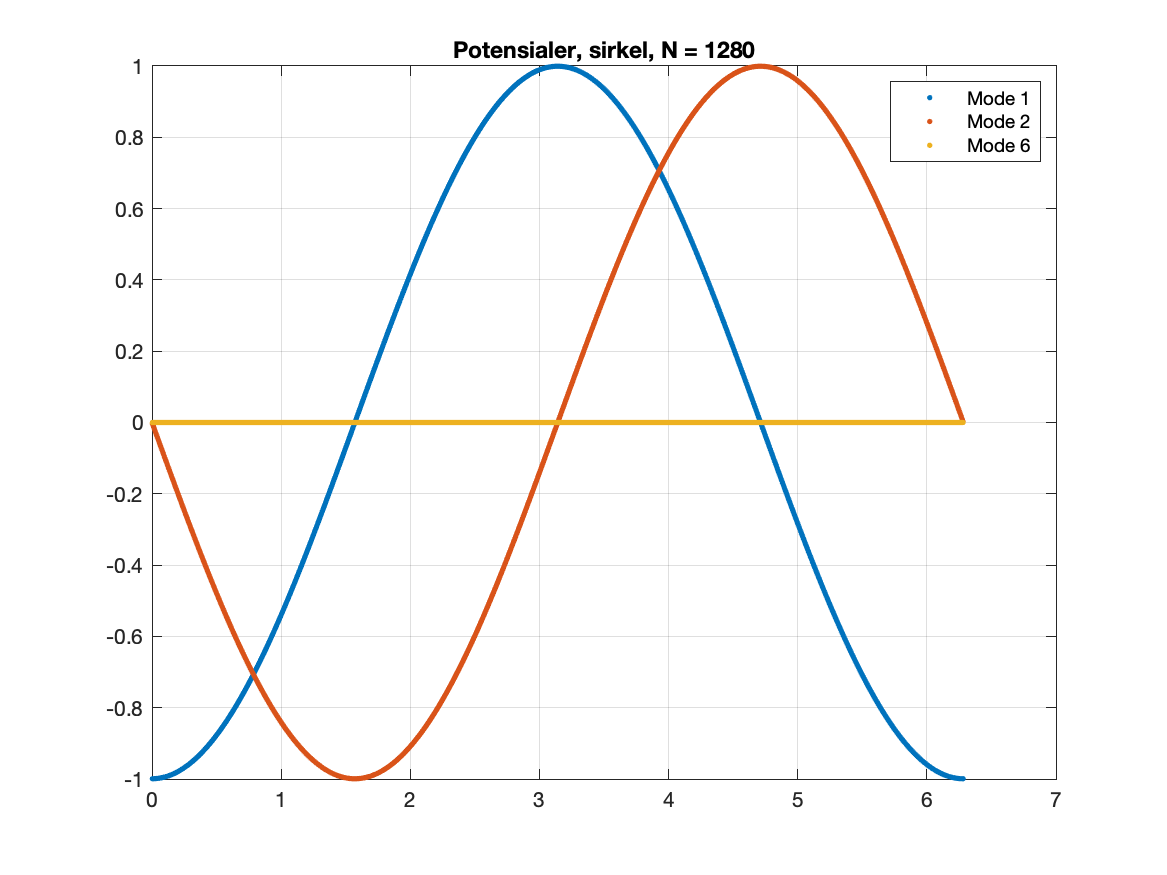
\includegraphics[width=0.8\linewidth]{/Users/ole/Tex/MEK4420/oblig1images/potensialer_sirkel.png}
%Vi ser at potensialene er identiske i fasong fra 0 til 2 pi, der mode 1 viser en minus cosinus-kurve, mode 2 en minus sinus kurve. Dvs at når sirkelen beveger seg horisontalt, mode 1, så er potensialet størst i bakkant, der sirkelen er =pi, og minst i front, eller høyre side =0=2pi. Denne sirkelen beveger seg altså til høyre. Rotasjon, mode 6 har intet potensial, ingen masse flyttes på når den glatte sirkelen roterer, så vi ser det stemmer at mode 6 er lik null.
\end{frame}

\begin{frame}
{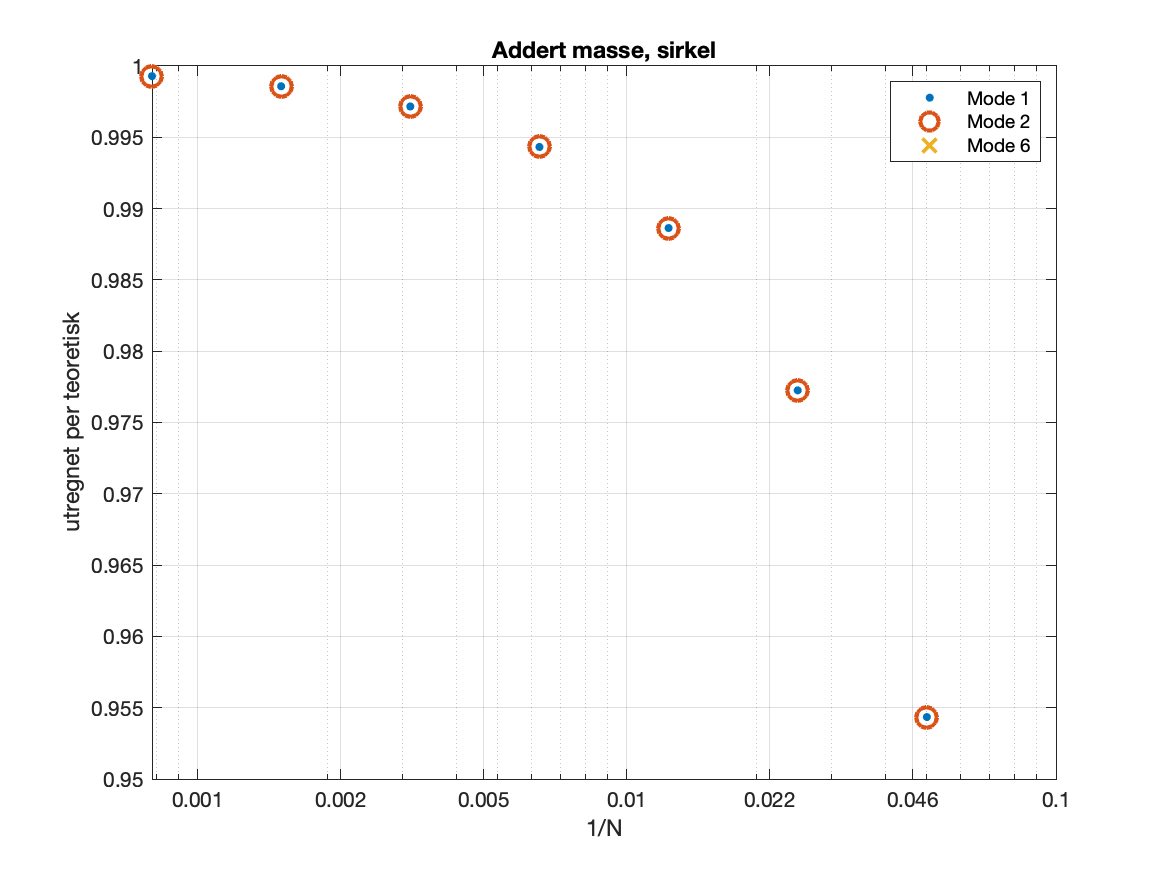
\includegraphics[width=0.8\linewidth]{/Users/ole/Tex/MEK4420/oblig1images/m11_sirkel.png}}
%Plott der vi sammenlikner den utregnede med teoretiske adderte massen. Vi ser et tydelig samsvar mellom teori og diskret utregning. En økning i N antall diskrete punkter viser at simulerte modellen nærmer seg den teoretiske. Sirkelen er symmetrisk, så horisontal og vertikal bevegelse gir nøyaktig samme adderte masse. 
Allerede ved første diskretisering, N=20, så har vi over 95\% samsvar mellom teoretisk og utregnet. 
%Som vi vil se i de neste plottene, varierer dette veldig mellom geometriene.
\end{frame}

% - - - Ellipse - - - %
\begin{frame}
%Vi tar en kjapp titt på diskretiseringen av ellipsen. Tilsynelatende bør vi bruke den jevne fordelingen, en vanlig ellipse merket med blå sirkler. Men den mer kompliserte inndelingen, merket med røde kryss, ble valgt fordi der endrer Arcustangens seg med en konstant verdi. 
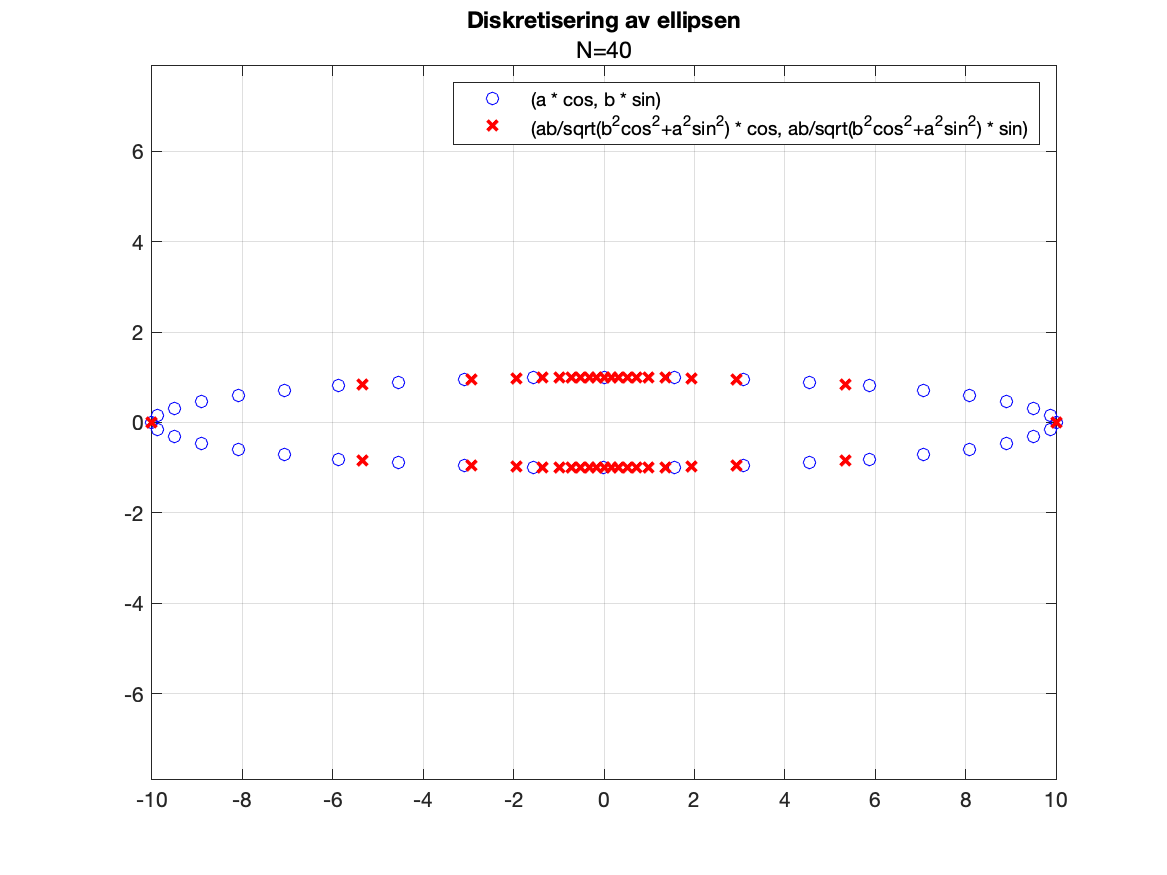
\includegraphics[width=0.8\linewidth]{/Users/ole/Tex/MEK4420/oblig1images/diskretisering_ellipse.png}
\end{frame}

\begin{frame}
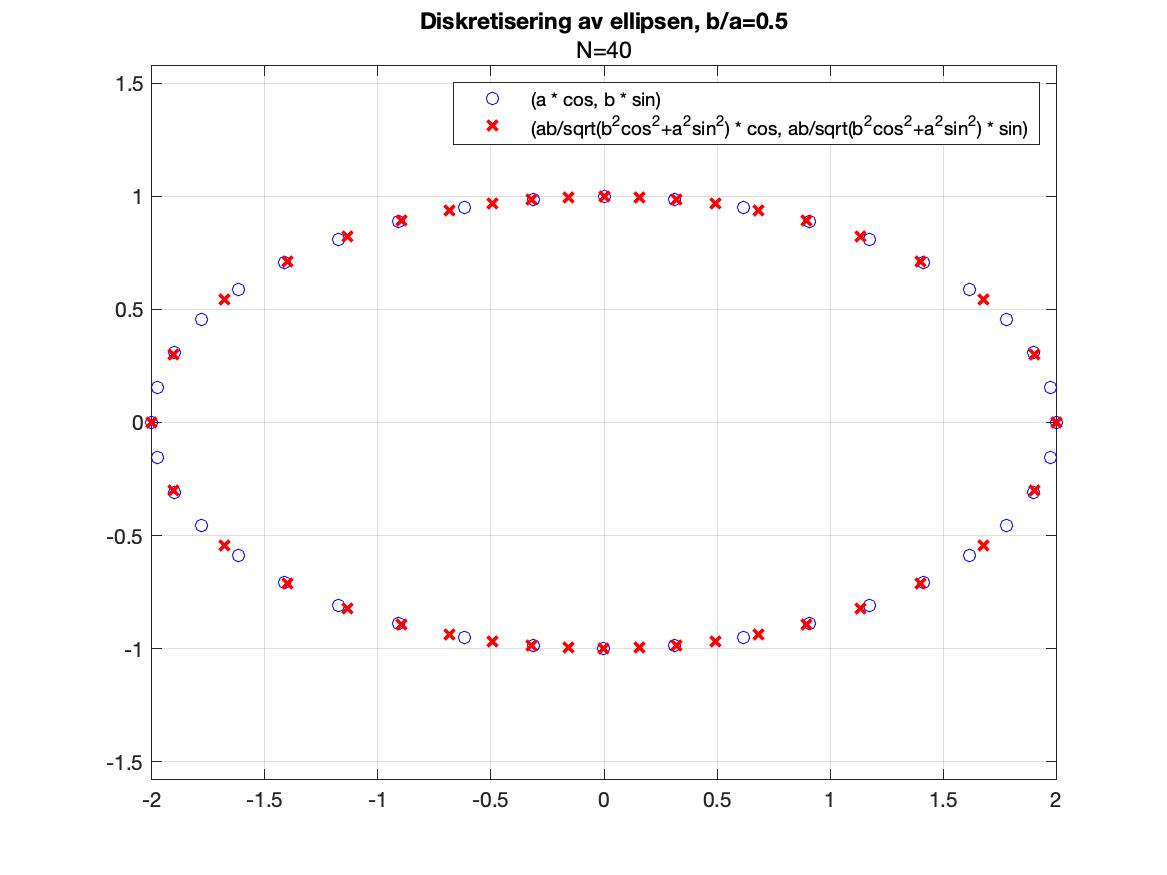
\includegraphics[width=0.8\linewidth]{/Users/ole/Tex/MEK4420/oblig1images/diskretisering_2ellipse.png}
\end{frame}

\begin{frame}
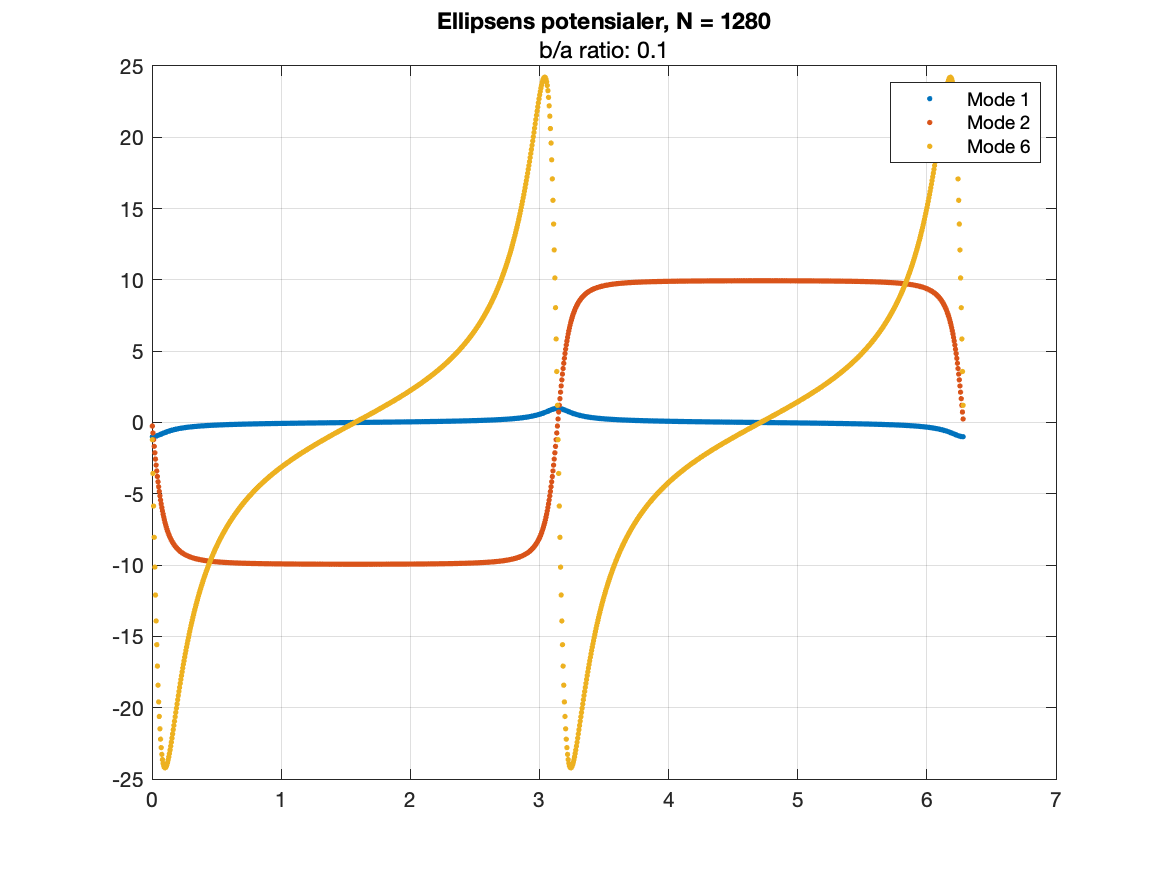
\includegraphics[width=0.8\linewidth]{/Users/ole/Tex/MEK4420/oblig1images/potensialer_ellipse.png}
%Ellipsens potensialer er svært ulike. Mode 1 har -1 i front og 1 i bakkant av ellipsen. Mode 2 har 10 ganger så mye, langs med toppen og bunnen. Rotasjonen, mode 6, viser svært stor respons på sidene av ellipsen. Som gir mening, det er ytterst på vår brede ellipse at mest vann fortrenges.
\end{frame}

\begin{frame}
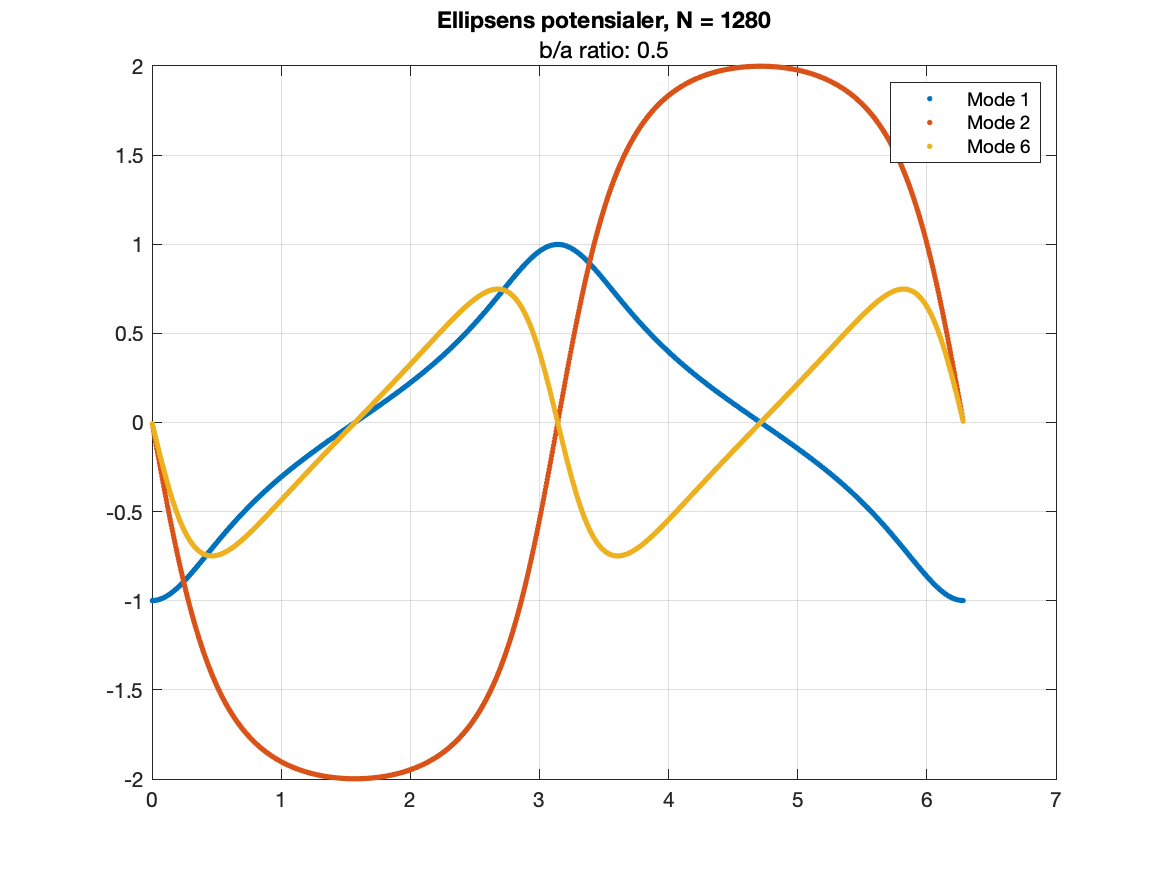
\includegraphics[width=0.8\linewidth]{/Users/ole/Tex/MEK4420/oblig1images/potensialer_2ellipse.png}
%For denne mer sirkulære ellipsen ser vi at den vertikale bevegelsen gir større forskjell i potensial enn rotasjonen.
\end{frame}

\begin{frame}
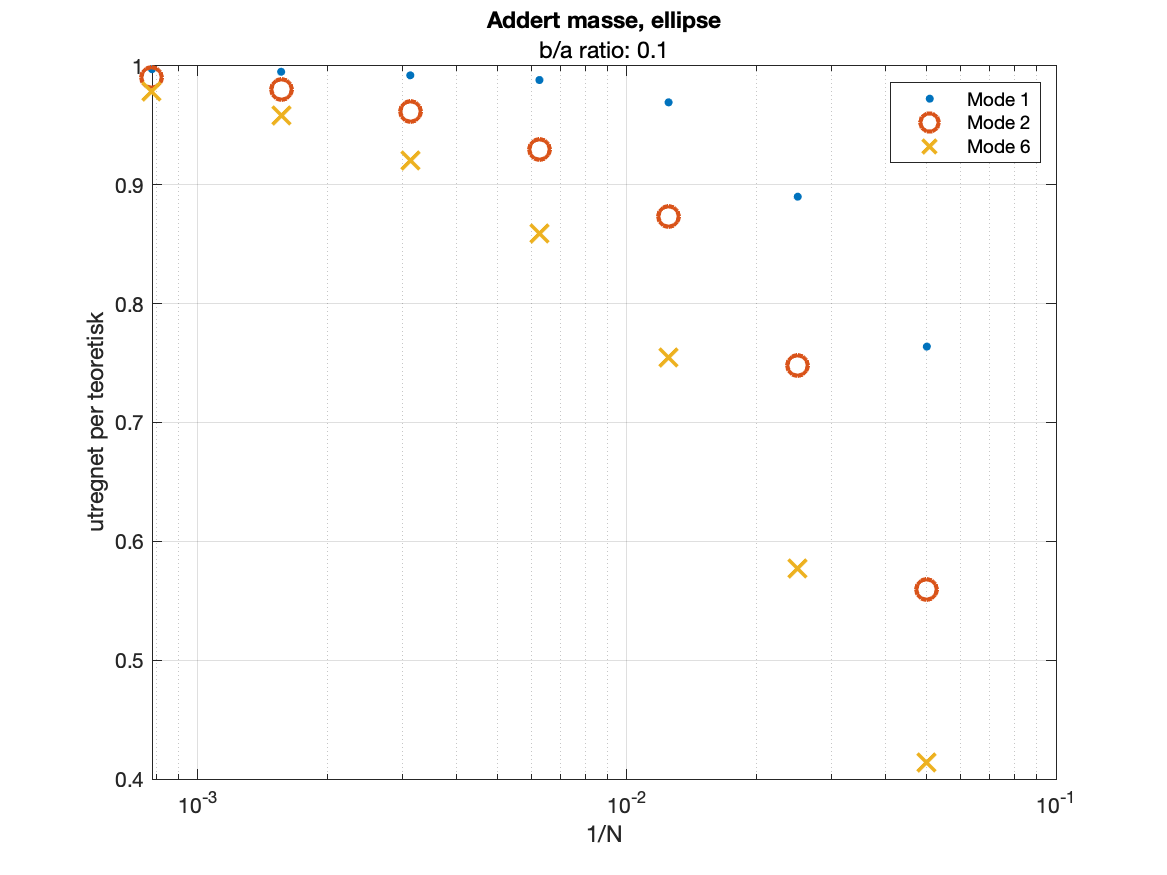
\includegraphics[width=0.8\linewidth]{/Users/ole/Tex/MEK4420/oblig1images/m11_ellipse.png}
%Vi sammenlikner utregnet og teoretisk addert masse for en bred ellipse. Bredden er 10x høyden. Vi ser at den horisontale bevegelsen, mode 1, trenger få punkter for at diskretiseringen skal samsvare godt med den teoretiske verdien. Vertikal bevegelse krever dobbelt så mange diskretiseringspunkter for tilsvarende samsvar. Rotasjon, mode 6, krever så omtrent dobbelt antall N som den vertikale, for tilsvarende samsvar. Verdier for 

N = 20,40,80,160,320,640,1280. 
\end{frame}

\begin{frame}
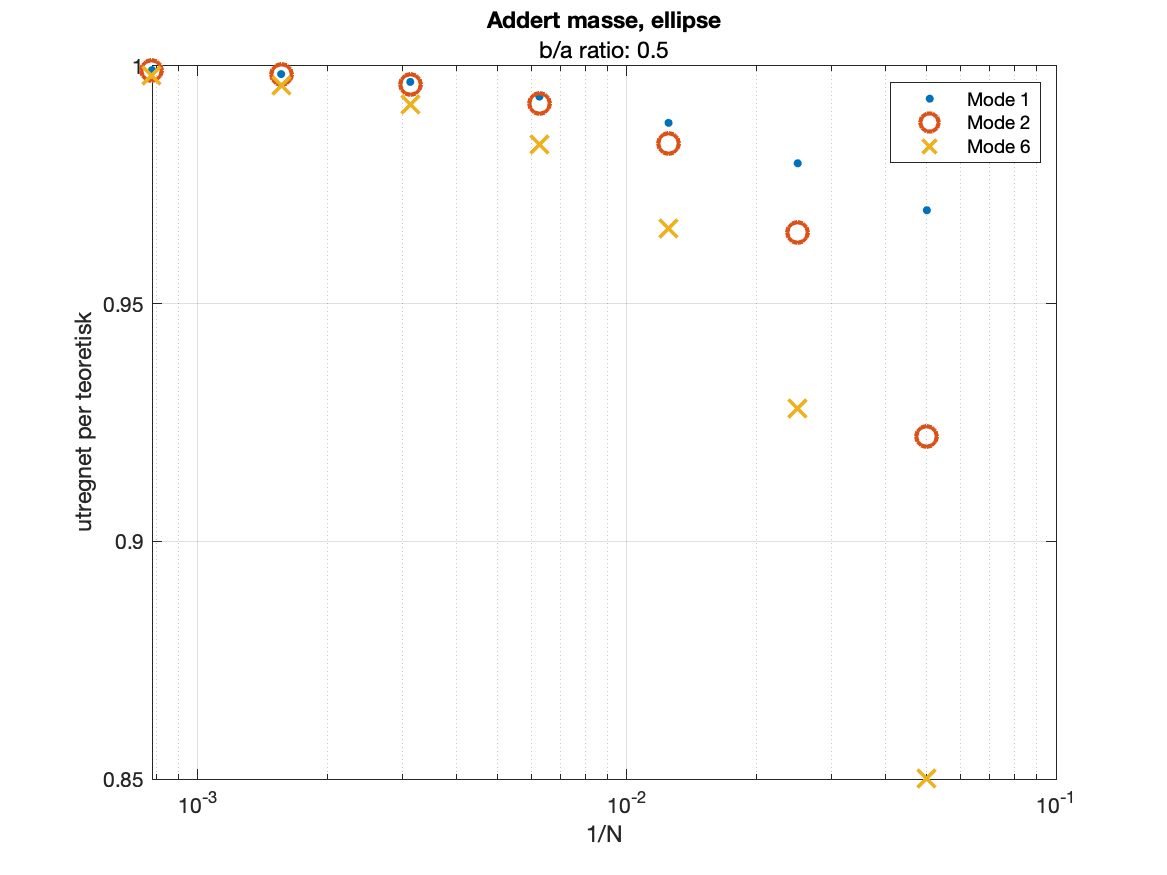
\includegraphics[width=0.8\linewidth]{/Users/ole/Tex/MEK4420/oblig1images/m11_2ellipse.png}
%Denne mer sirkulære ellipsen trenger mye færre punkter for å oppnå samme samsvar mellom teoretisk og utregnet addert masse. Over 95\% samsvar etter bare 20, 40 og 80 punkter for henholdsvis mode 1, 2 og 6.

N = 20,40,80,160,320,640,1280.
\end{frame}




% - - - KVADRAT - - - %
\begin{frame}
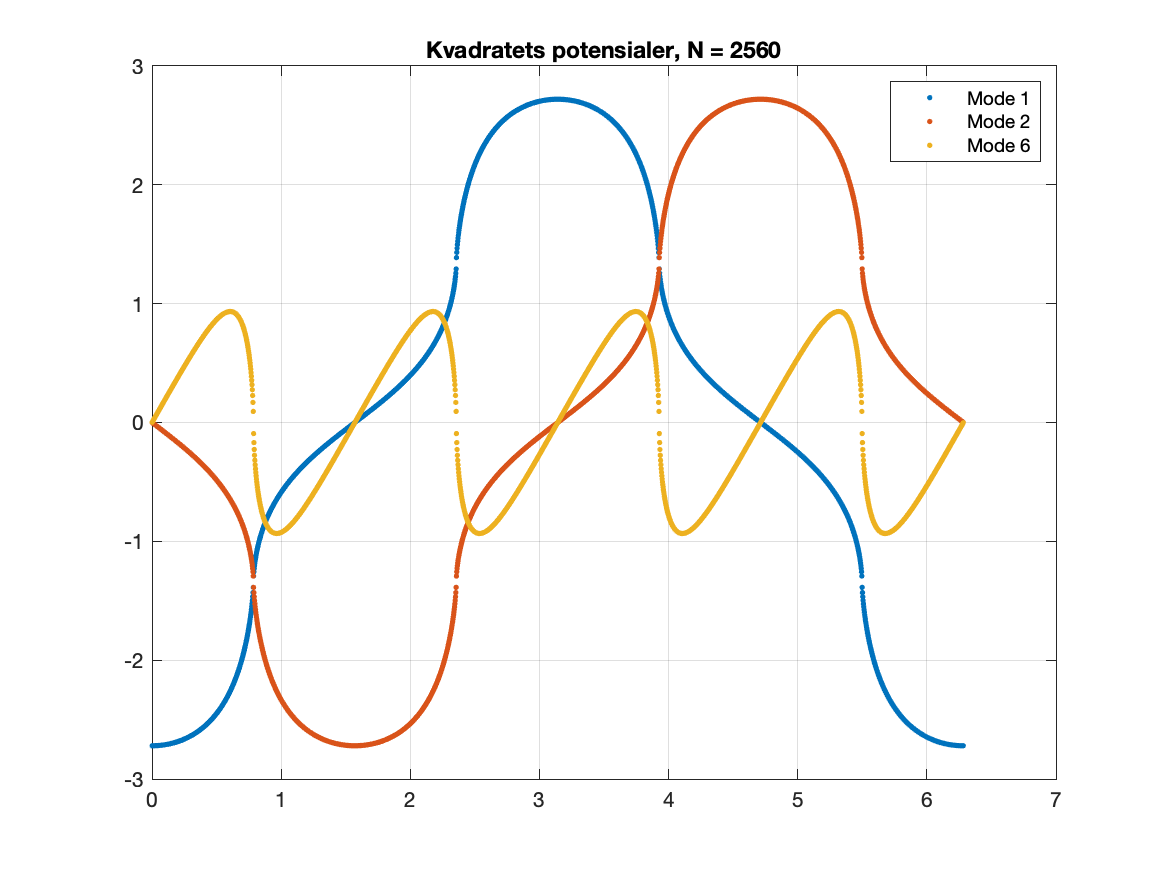
\includegraphics[width=0.8\linewidth]{/Users/ole/Tex/MEK4420/oblig1images/potensialer_kvadrat.png}
%Kvadratets potensialer i horisontal og vertikal retning er like. Rotasjonen viser tydelig samme utslag ved hvert hjørne
\end{frame}
\begin{frame}
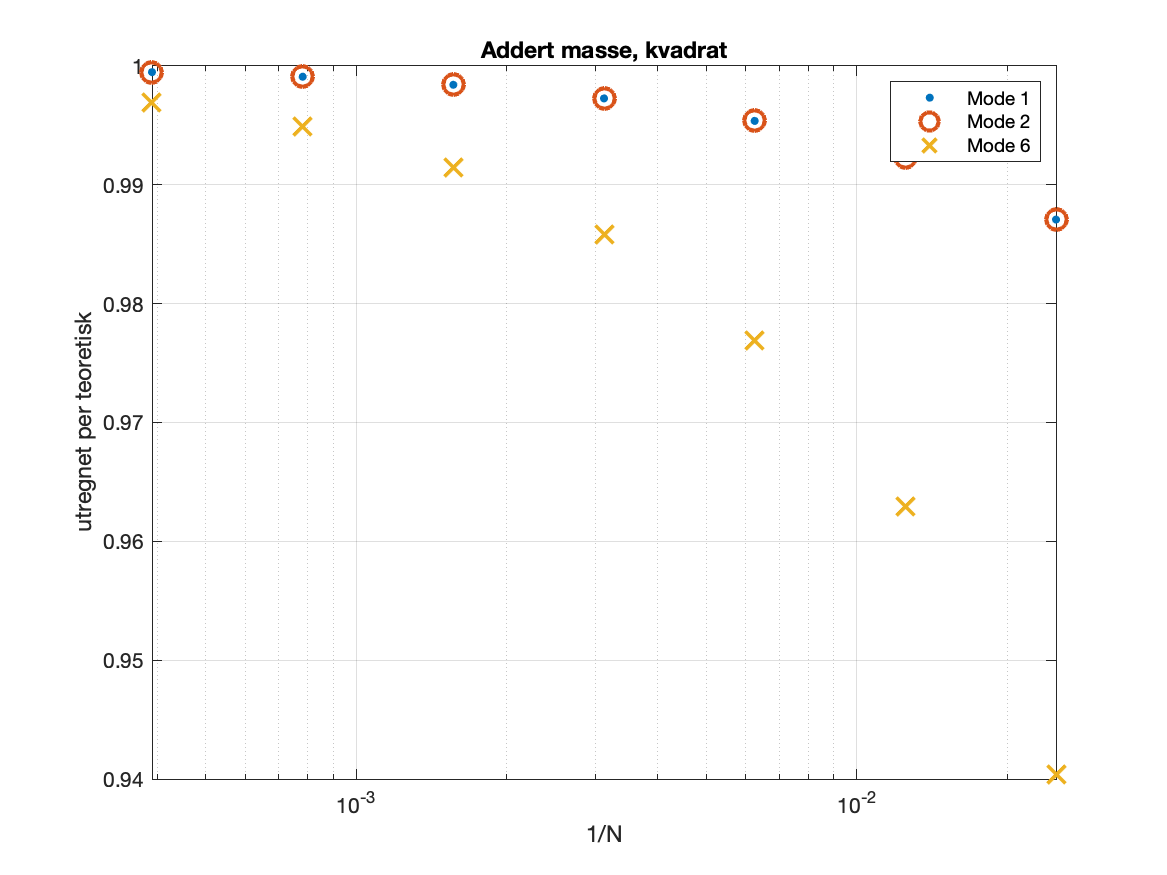
\includegraphics[width=0.8\linewidth]{/Users/ole/Tex/MEK4420/oblig1images/m11_kvadrat.png}
%På kvadratet har det blitt brukt ett hakk flere N. Verdier for
 
N = 40,80,160,320,640,1280,2560.
\end{frame}


\begin{frame}
Vi har sett på 3 geometrier: sirkel, ellipse, og kvadrat. Vi har sett at den utregnede adderte massen konvergerer mot den teoretiske, med ulik hastighet, når vi øker N diskretiseringspunkter. Det er fasongen på geometrien som avgjør responsen. 
\end{frame}




%%%%%%%%%%%%%%%%%%%%%%%%%%%%
%%%%%%%%%%% ... DEL 2 ... %%%%%%%%%%%
%%%%%%%%%%%%%%%%%%%%%%%%%%%%
\section{Del 2 - Krefter og respons i hiv}
\subsection{Randverdier}
\begin{frame}
  \frametitle{Randverdiene for problemet}
  \begin{enumerate}
  \item Kinematisk grensebetingelse
  \item uendelig dyp.
  \item innkompressibelt, uten virvling. Laplace.      
  \end{enumerate}
\end{frame}
% - % - % - % - % - %
\begin{frame}
  \frametitle{Randverdiene for Green-funksjonen}
  \begin{enumerate}
  \item      
  \end{enumerate}
\end{frame}

\subsection{Diskretisering}
\begin{frame}{}
    % First Row
    \begin{minipage}[t]{0.45\linewidth}
        \centering
        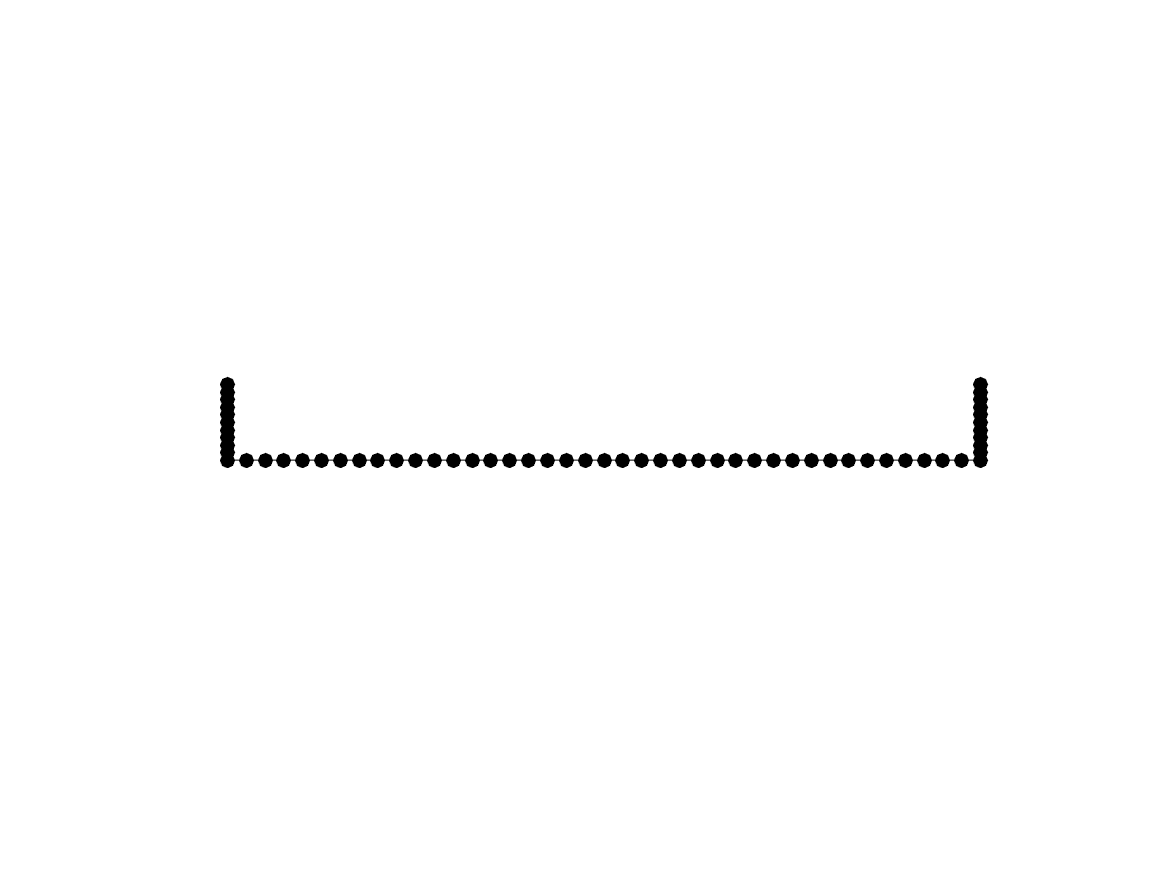
\includegraphics[width=\linewidth]{/Users/ole/Tex/MEK4420/oblig2images/boxes_1.png}
        \captionof{figure}{L/D = 10}
    \end{minipage}%
    \hspace{0.05\linewidth}  % Spacing between images
    \begin{minipage}[t]{0.45\linewidth}
        \centering
        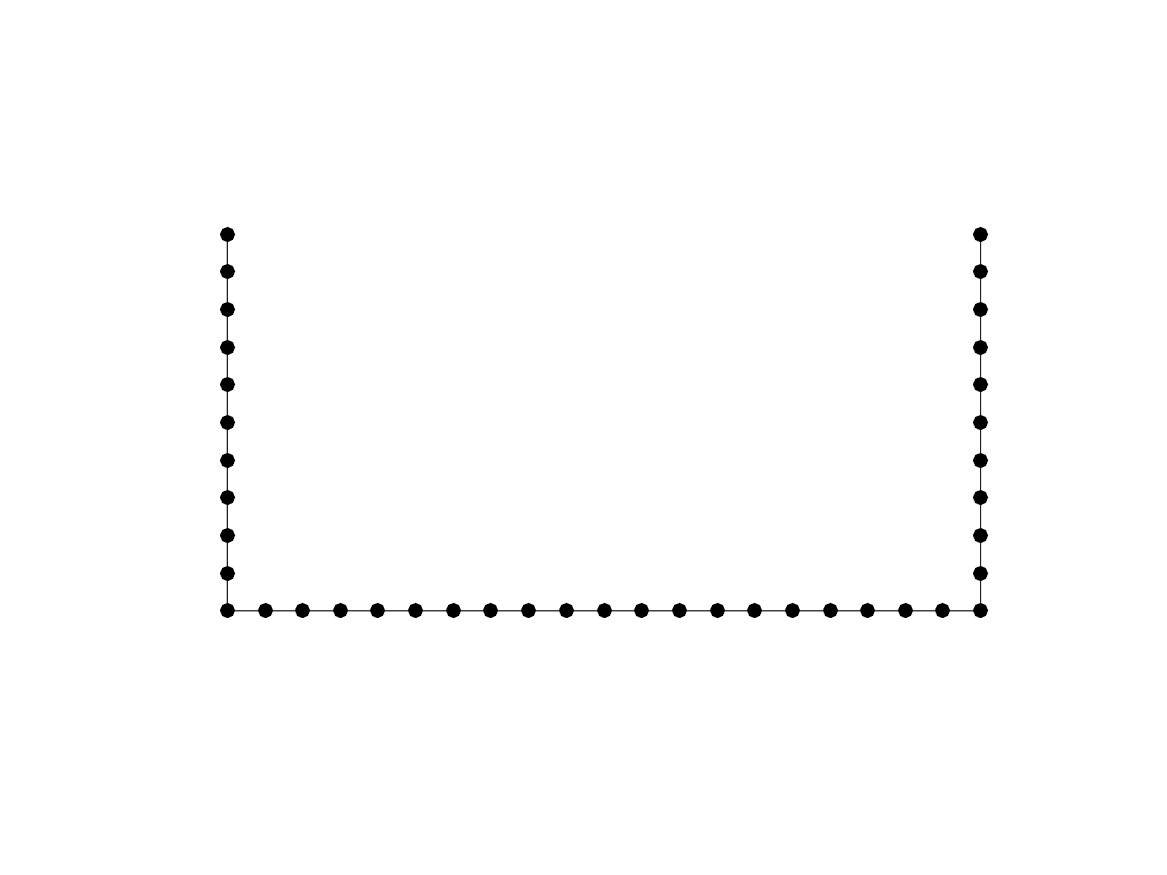
\includegraphics[width=\linewidth]{/Users/ole/Tex/MEK4420/oblig2images/boxes_2.png}
        \captionof{figure}{L/D = 2}
    \end{minipage}

    \vspace{-0.2cm}  % Adjust vertical space for overlap

    % Second Row
    \begin{minipage}[t]{0.45\linewidth}
        \centering
        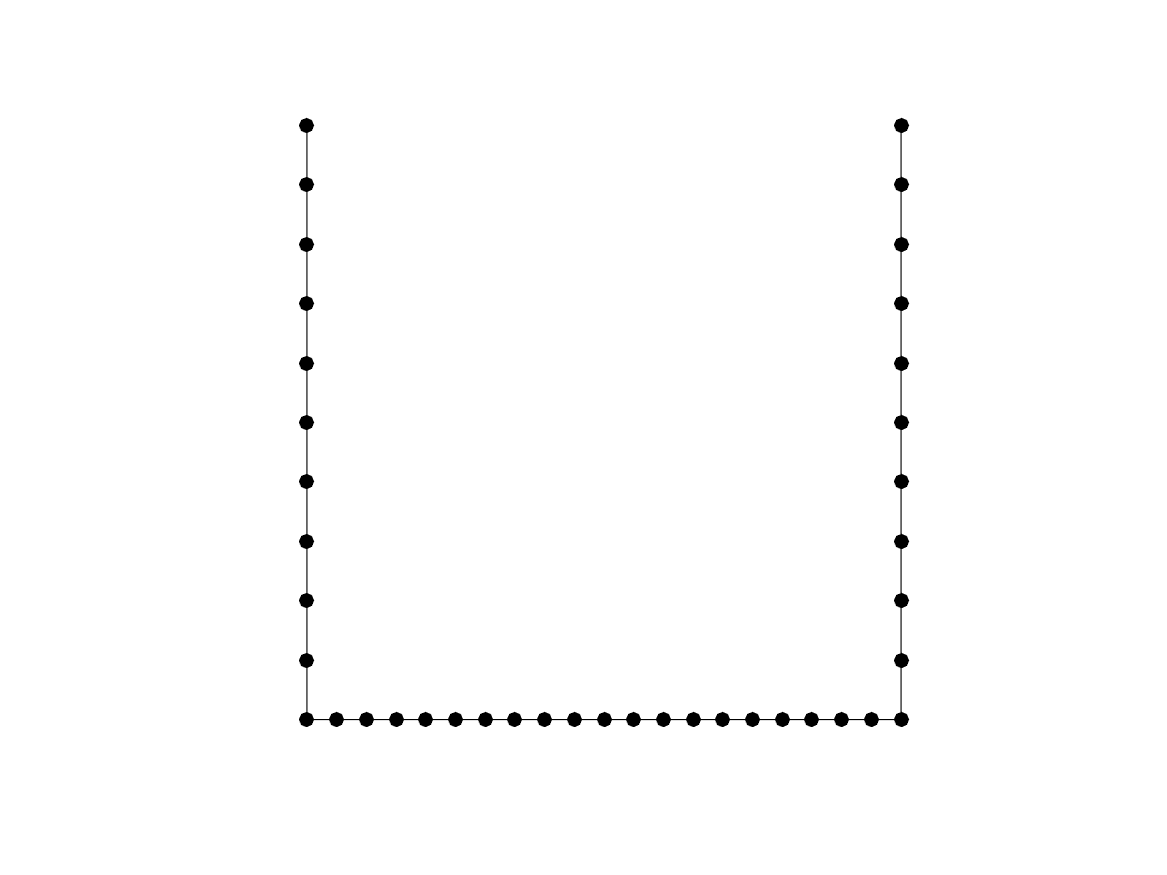
\includegraphics[width=\linewidth]{/Users/ole/Tex/MEK4420/oblig2images/boxes_3.png}
        \captionof{figure}{L/D = 1}
    \end{minipage}%
    \hspace{0.05\linewidth}  % Spacing between images
    \begin{minipage}[t]{0.45\linewidth}
        \centering
        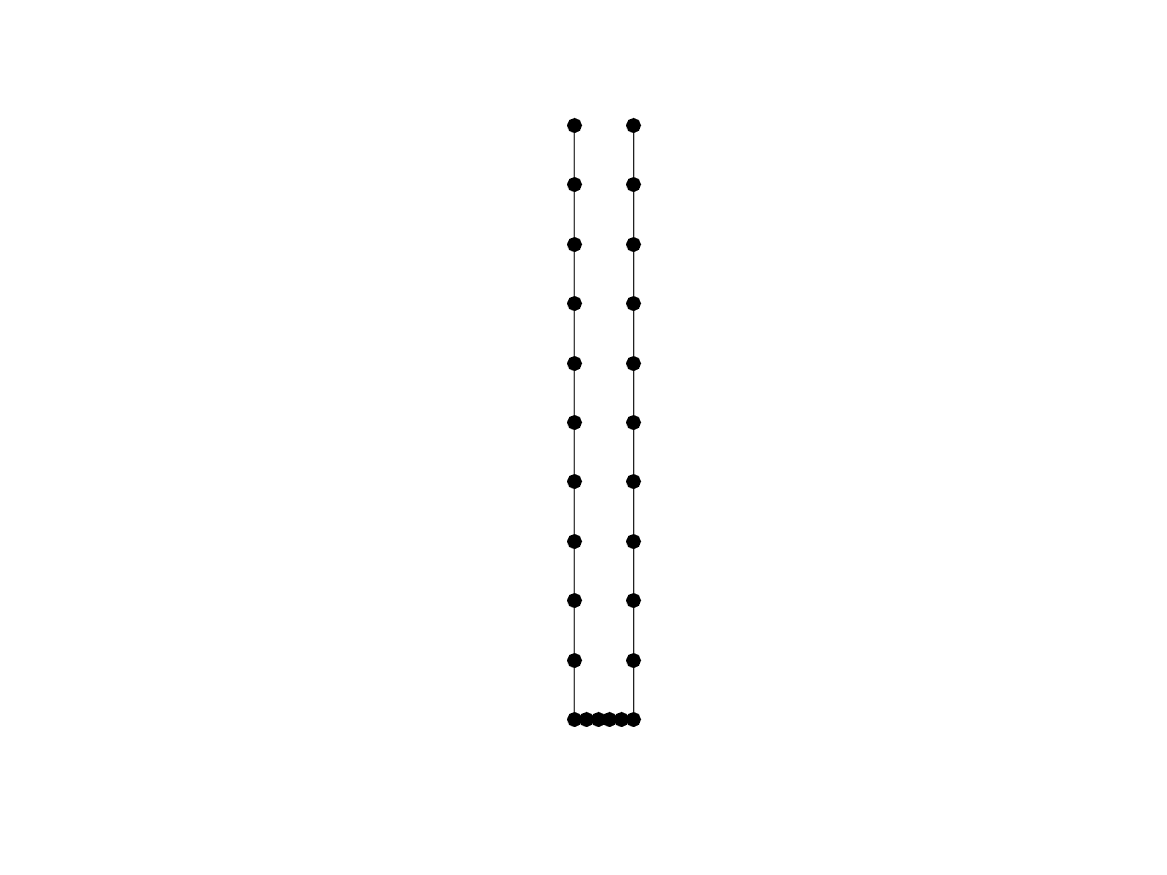
\includegraphics[width=\linewidth]{/Users/ole/Tex/MEK4420/oblig2images/boxes_4.png}
        \captionof{figure}{L/D = 0.1}
    \end{minipage}
\end{frame}

\begin{frame}
Vi ønsker å løse integrallikningen:
\begin{equation}\label{eq:144}
    -\pi \phi_2  + \int_{S_B} \phi_2 \frac{\partial G}{\partial n}  dS = \int_{S_B} G n_2 dS
\end{equation}
Men før vi gjør det vil vi sjekke at likningen fungerer. Så vi løser høyre- og venstresiden av en integrallikning der vi kjenner alle variablene. Vi ønsker å se om den reelle delen til høyresiden tilsvarer den reelle delen til venstresiden, og tilsvarende for de imaginære delene. 
\end{frame}

%her er det mulig å lime inn mere tekst og likninger.

%\subsection{Vi tester den numeriske løseren med KD=0.9}
\begin{frame}
\begin{minipage}[t]{0.45\linewidth}
    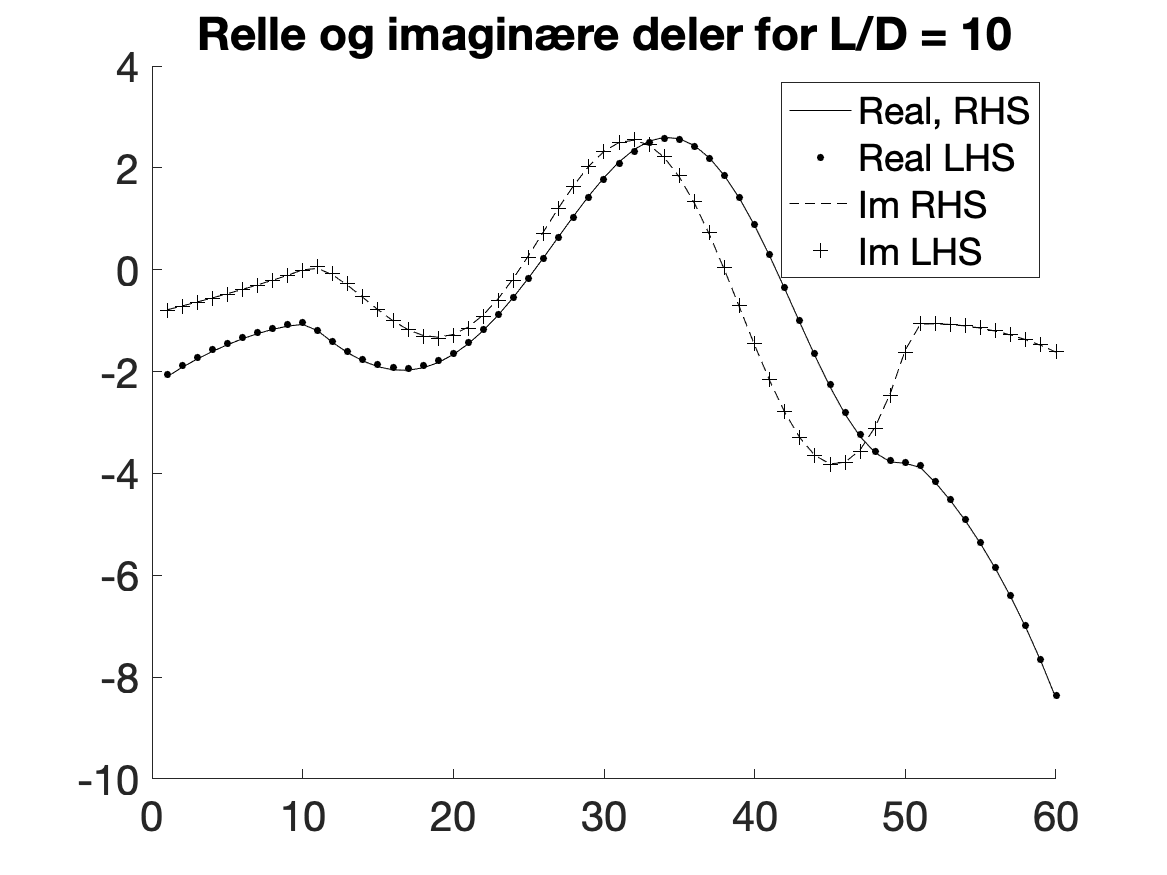
\includegraphics[width=\linewidth]{/Users/ole/Tex/MEK4420/oblig2images/plot_1_LD_1_nu09.png}
    \captionof{figure}{L/D = 10}
\end{minipage}
\hspace{0.05\linewidth}
\begin{minipage}[t]{0.45\linewidth}
    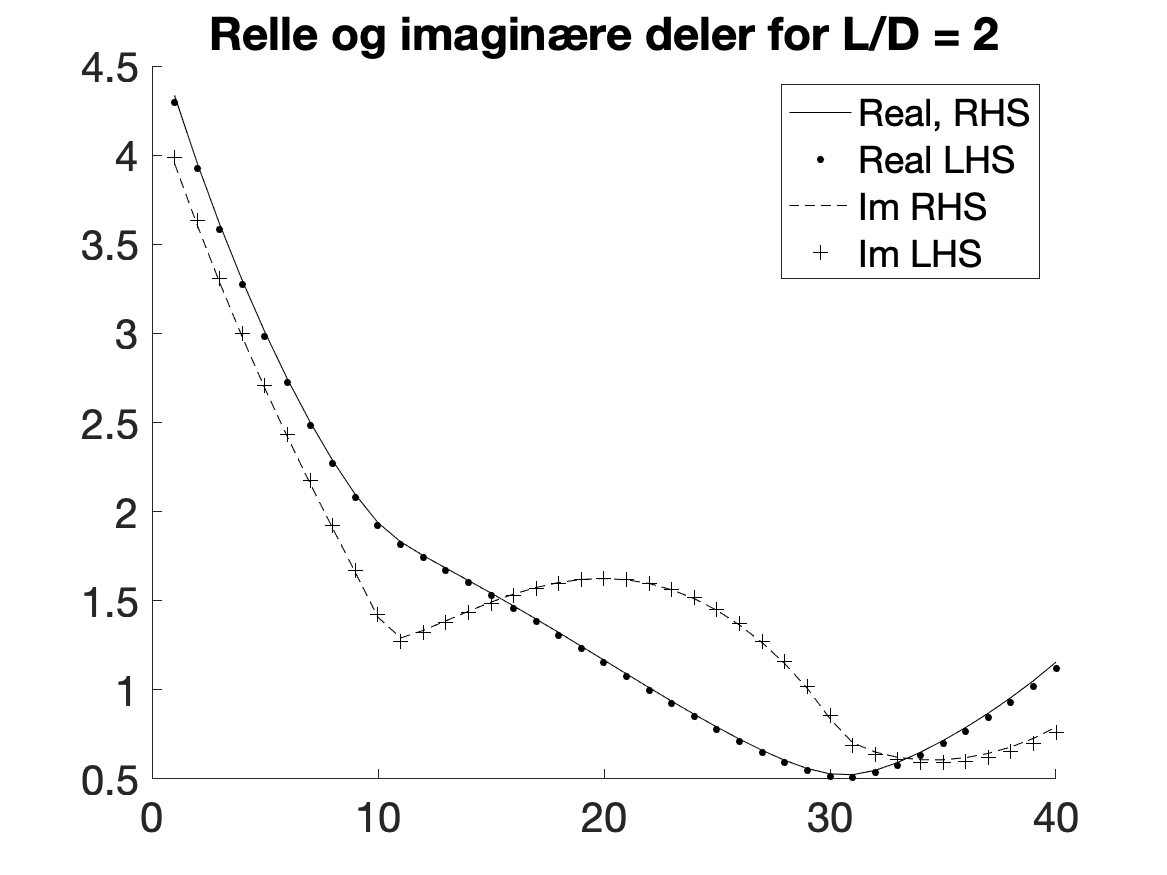
\includegraphics[width=\linewidth]{/Users/ole/Tex/MEK4420/oblig2images/plot_2_LD_2_nu09.png}
    \captionof{figure}{L/D = 2}
\end{minipage}
\begin{minipage}[t]{0.45\linewidth}
    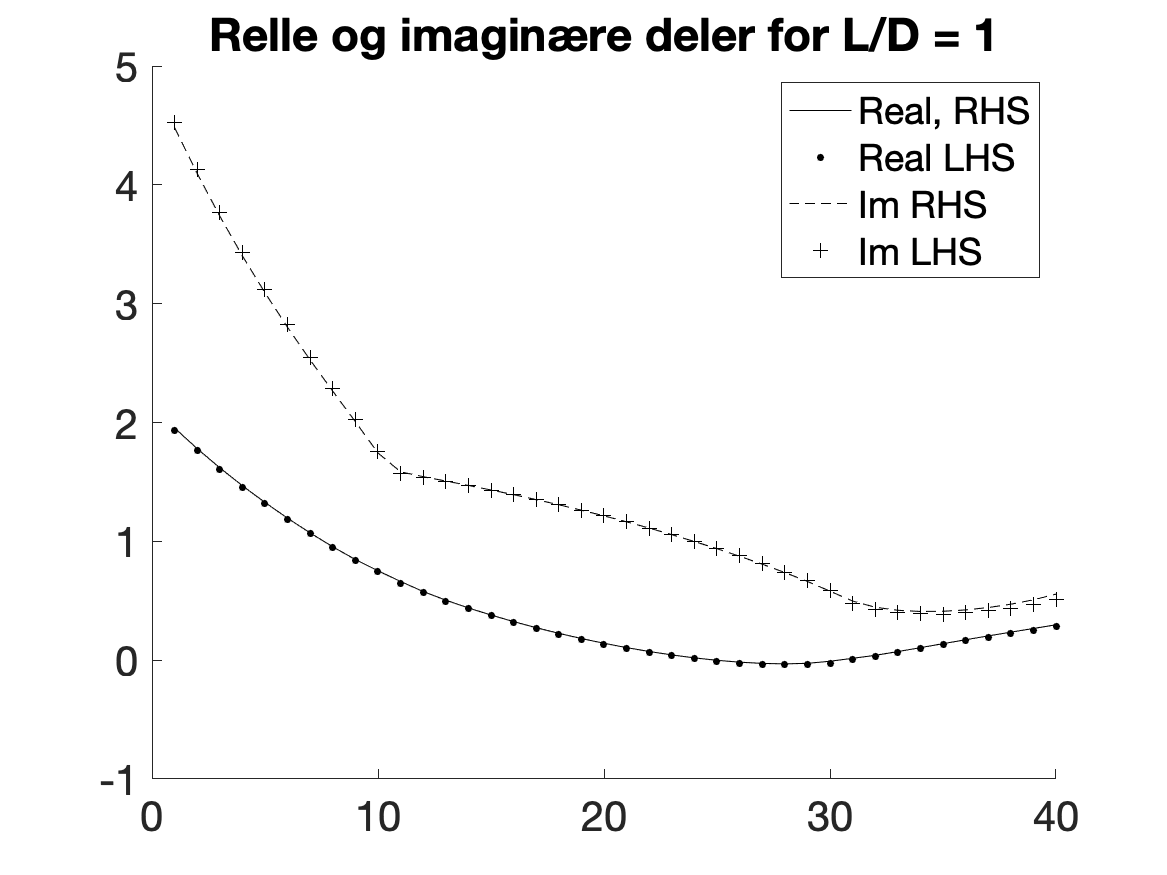
\includegraphics[width=\linewidth]{/Users/ole/Tex/MEK4420/oblig2images/plot_3_LD_3_nu09.png}
    \captionof{figure}{L/D = 1}
\end{minipage}
\hspace{0.05\linewidth}
\begin{minipage}[t]{0.45\linewidth}
    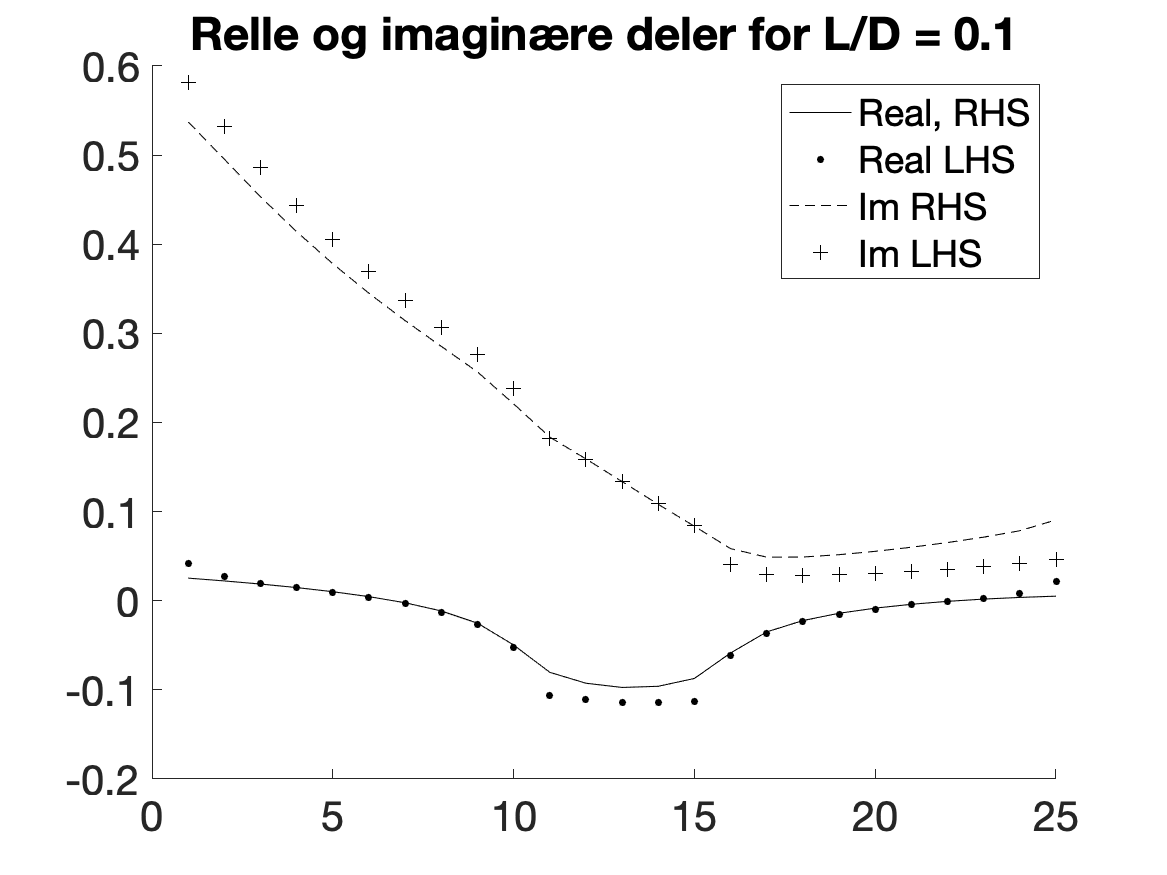
\includegraphics[width=\linewidth]{/Users/ole/Tex/MEK4420/oblig2images/plot_4_LD_4_nu09.png}
    \captionof{figure}{L/D = 0.1}
\end{minipage}
\end{frame}

%\subsection{Vi tester den numeriske løseren med KD=1.2}
\begin{frame}
\begin{minipage}[t]{0.45\linewidth}
    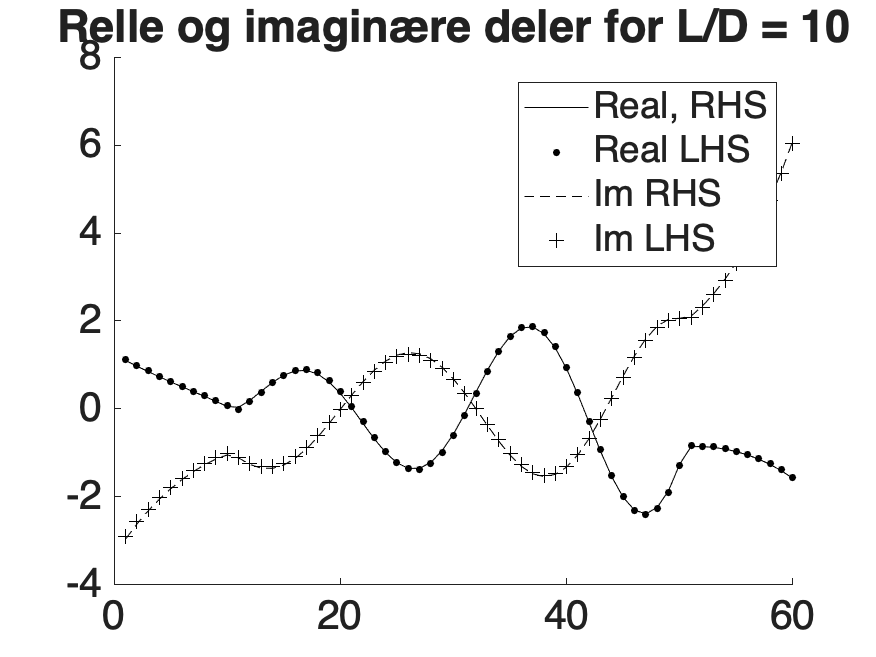
\includegraphics[width=\linewidth]{/Users/ole/Tex/MEK4420/oblig2images/plot_1_LD_1_nu12.png}
    \captionof{figure}{L/D = 10}
\end{minipage}
\hspace{0.05\linewidth}
\begin{minipage}[t]{0.45\linewidth}
    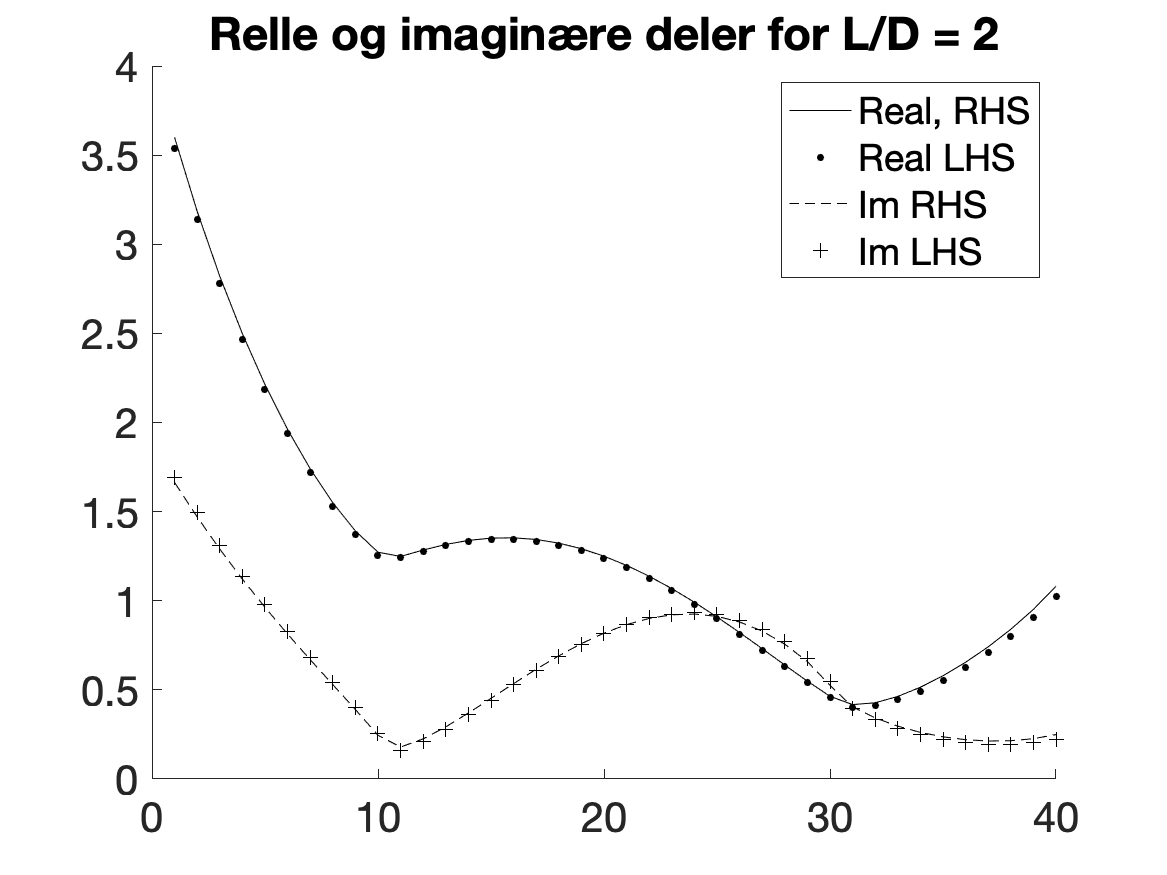
\includegraphics[width=\linewidth]{/Users/ole/Tex/MEK4420/oblig2images/plot_2_LD_2_nu12.png}
    \captionof{figure}{L/D = 2}
\end{minipage}
\begin{minipage}[t]{0.45\linewidth}
    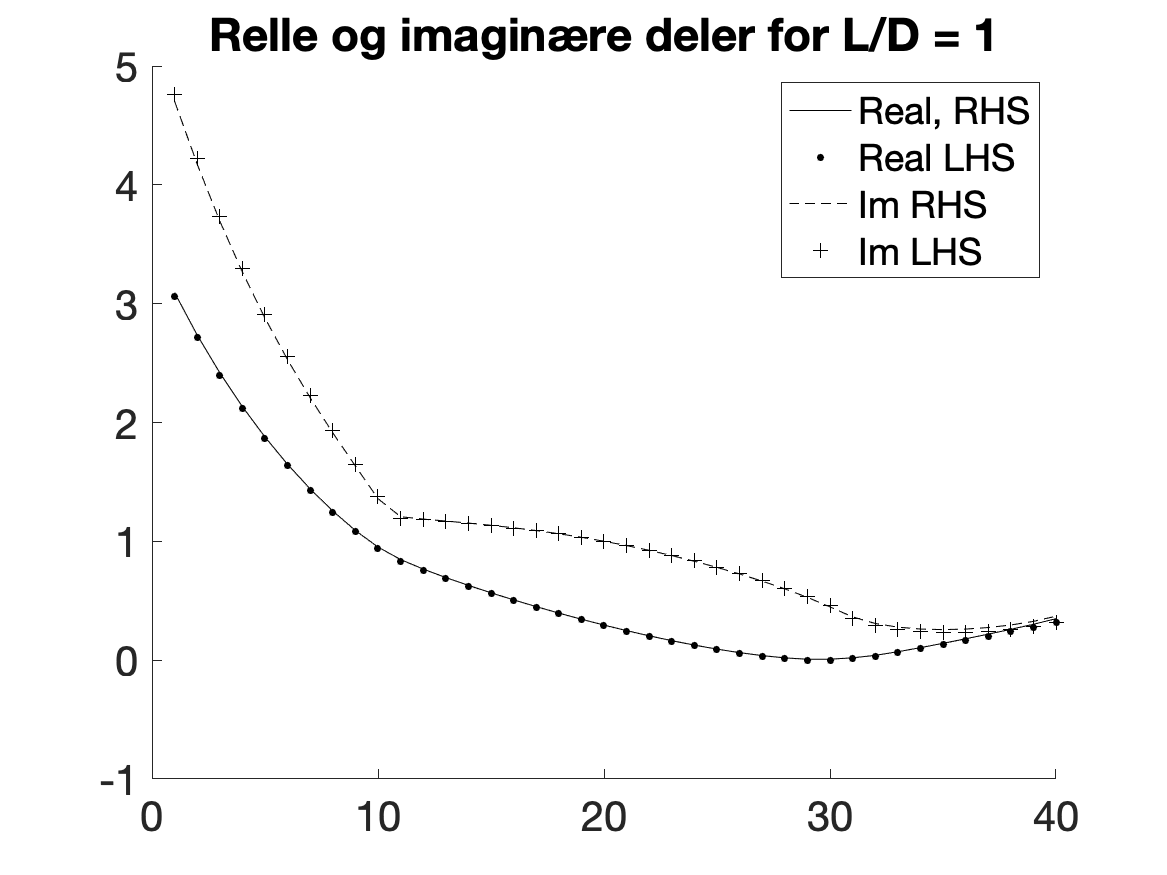
\includegraphics[width=\linewidth]{/Users/ole/Tex/MEK4420/oblig2images/plot_3_LD_3_nu12.png}
    \captionof{figure}{L/D = 1}
\end{minipage}
\hspace{0.05\linewidth}
\begin{minipage}[t]{0.45\linewidth}
    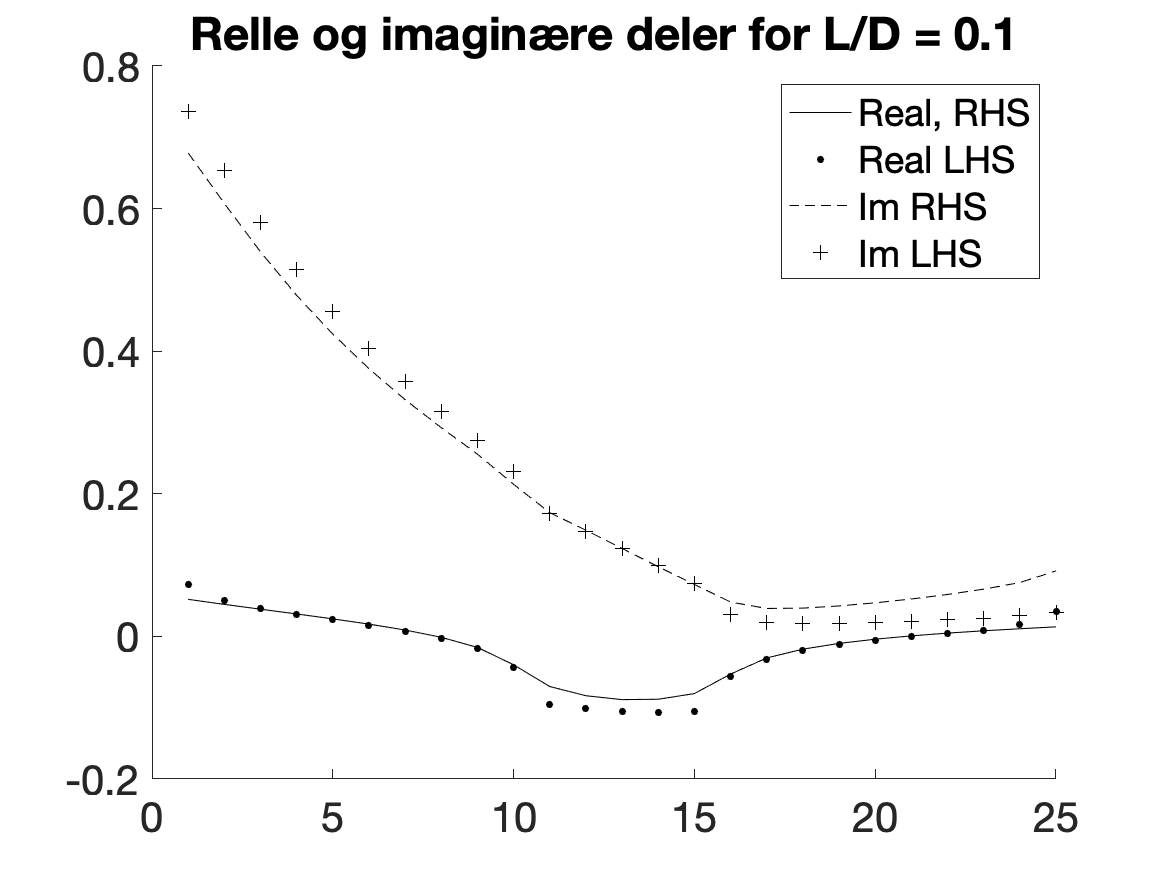
\includegraphics[width=\linewidth]{/Users/ole/Tex/MEK4420/oblig2images/plot_4_LD_4_nu12.png}
    \captionof{figure}{L/D = 0.1}
\end{minipage}
\end{frame}

% 7.5.3 Løsning av problemet i hiv
\begin{frame}
%Så løser vi den originale likningen (\ref{eq:144}) numerisk for alle 4 geometriene. Og ser på plott av verdiene for potensialet $\phi_2$ på y-aksen. På x-aksen har vi de diskrete punktene. Plottet er symmetrisk fordi geometrien er symmetrisk.
\begin{minipage}[t]{0.45\linewidth}
    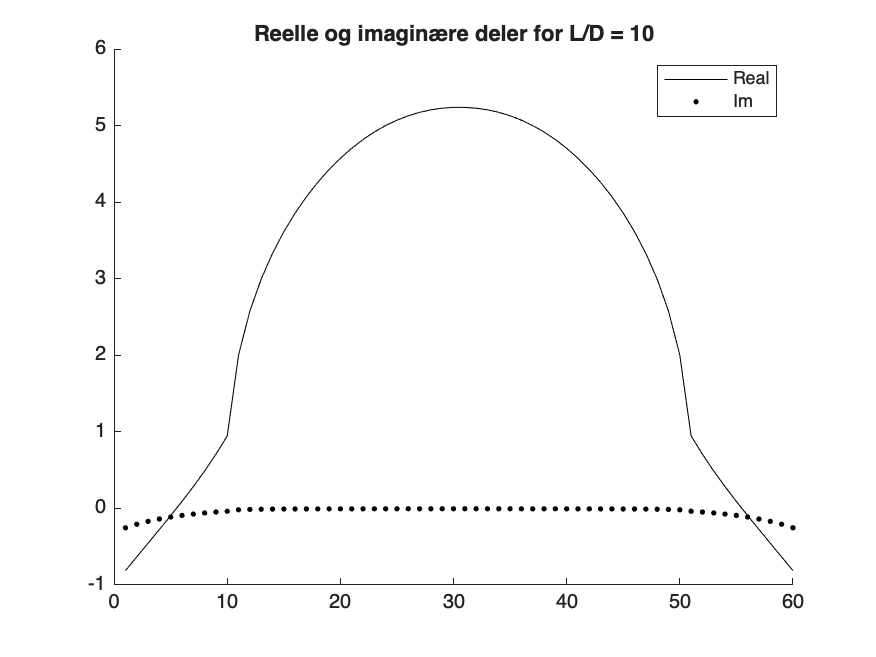
\includegraphics[width=\linewidth]{/Users/ole/Tex/MEK4420/oblig2images/plot_phi2_1.png}
    \captionof{figure}{L/D = 10}
\end{minipage}
\hspace{0.05\linewidth}
\begin{minipage}[t]{0.45\linewidth}
    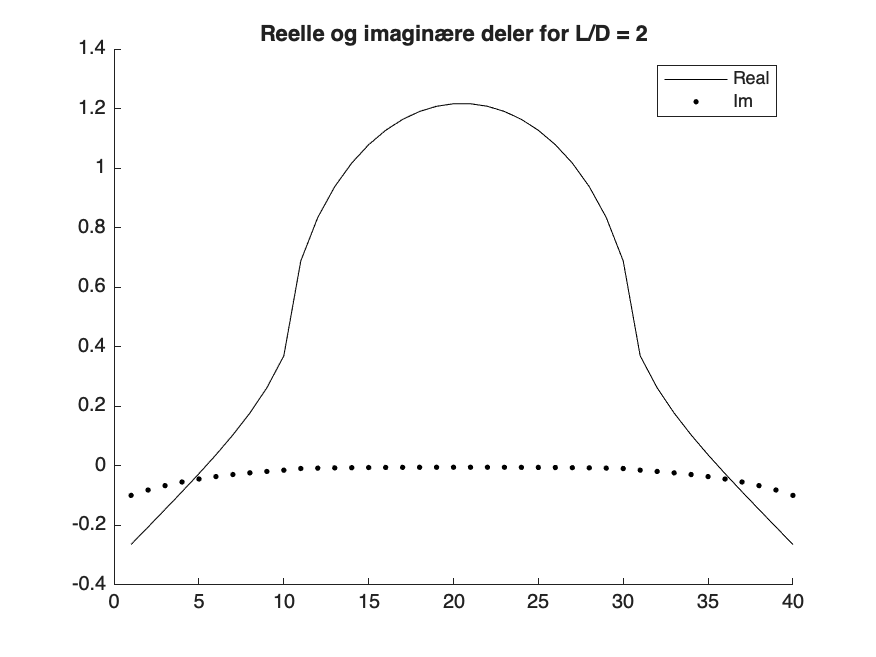
\includegraphics[width=\linewidth]{/Users/ole/Tex/MEK4420/oblig2images/plot_phi2_2.png}
    \captionof{figure}{L/D = 2}
\end{minipage}
\begin{minipage}[t]{0.45\linewidth}
    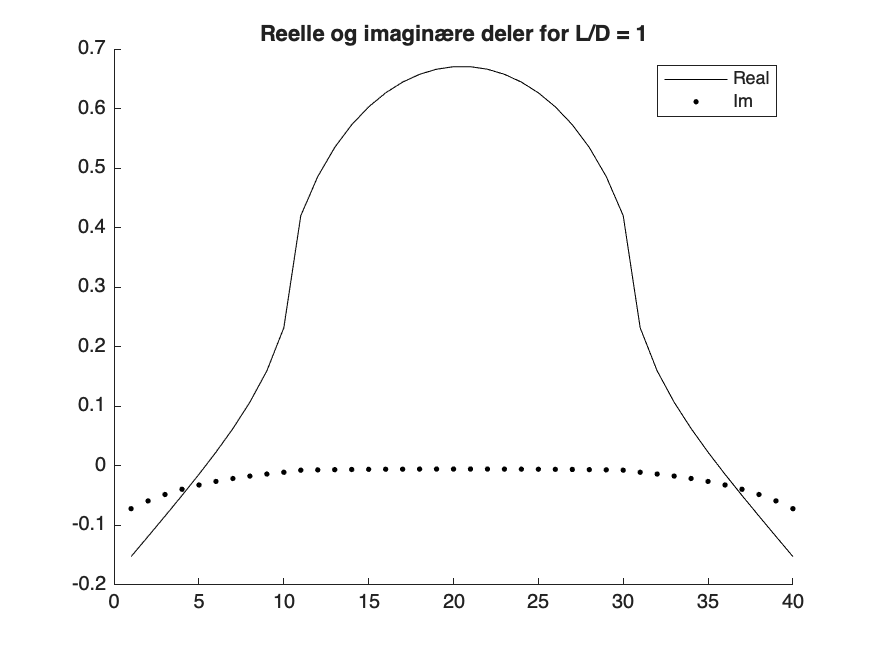
\includegraphics[width=\linewidth]{/Users/ole/Tex/MEK4420/oblig2images/plot_phi2_3.png}
    \captionof{figure}{L/D = 1}
\end{minipage}
\hspace{0.05\linewidth}
\begin{minipage}[t]{0.45\linewidth}
    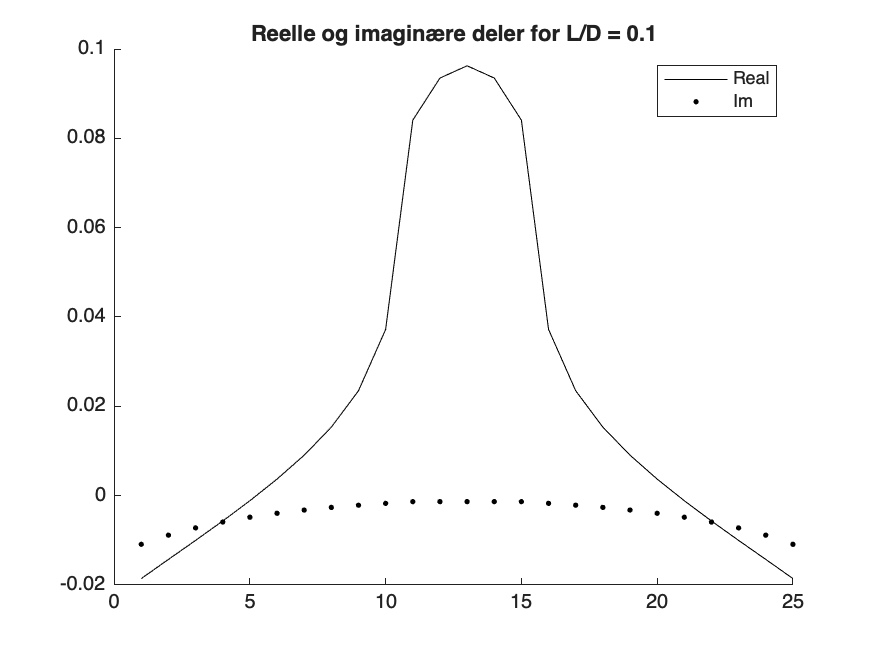
\includegraphics[width=\linewidth]{/Users/ole/Tex/MEK4420/oblig2images/plot_phi2_4.png}
    \captionof{figure}{L/D = 0.1}
\end{minipage}
\end{frame}

% 7.6 - Potensialet i fjernfeltet
\begin{frame}
Langt borte, når for $\bar{x} \rightarrow \pm \infty$ har potensialet $\phi_2$  denne formen
\begin{align}
	\phi_2(\bar{x},\bar{y}) &\rightarrow A_2^{-\infty} e^{K\bar{y} + \mathrm{i} K\bar{x}}, \quad \bar{x} \rightarrow -\infty, \\
	\phi_2(\bar{x},\bar{y}) &\rightarrow A_2^{\infty} e^{K\bar{y} - \textsf{i} K\bar{x}}, \qquad \bar{x} \rightarrow \infty,
\end{align}
der $K = \frac{\omega^2}{g}$

fra likningen for fluidet så kan vi finne $A_2^{-\infty}$ og $A_2^{\infty}$
\begin{equation}
    2\pi \phi_2(\bar{x},\bar{y})  = \int_{S_B}  ( \phi_2  \frac{\partial G }{\partial n}-G n_2 )dS
\end{equation}

%avskrift fra side 32.
oppførselen til $\phi_j$ for $\bar{x} \rightarrow \pm \infty$,
\begin{align}
\phi_2 \rightarrow A_2^{\pm \infty} e^{K (\bar{y} \mp \mathrm{i}  \bar{x}) }, \quad \bar{x} \rightarrow \pm \infty.
\end{align}
%her har jeg byttet tre subscript fra j til 2.
Der de komplekse konstantene $A_2^{\pm \infty}$ finnes ved å ta integralet over svømmeflaten, som gir
\begin{align}
A_2^{\pm \infty} = \mathrm{i} \int_{S_B} \bigg(\phi_2 (n_1 \frac{\partial}{\partial x} + n_2  \frac{\partial}{\partial y}) - n_2 \bigg) e^{K(\bar{y} \pm \mathrm{i} \bar{x})} dS
\end{align}
\end{frame}

% 7.7 utgående bølgeamplitude 
\begin{frame}
Den utgående bølgeamplituden har komplekse amplituder,
\begin{align}
	amp_2^{\infty} = \xi_2 A_j^{ \infty} \frac{\omega^2}{g}, \quad \text{og} \quad amp_2^{-\infty} = \xi_2 A_j^{- \infty} \frac{\omega^2}{g}.
\end{align}
Gjennomsnittet av energifluksen til den utgående bølgen er gitt ved
\begin{align}
	\overline{\text{Energifluks}} = \bar{E}^{\infty}c_g + \bar{E}_j^{-\infty}c_g =  \frac{1}{2}\rho g {|amp_2|}^{\infty}c_g + \frac{1}{2}\rho g {|amp_2|}^{-\infty}c_g,
\end{align}
der $\bar{E}^{\pm \infty}$ er gjennomsnittlig energitetthet til utgående bølger og $c_g = \frac{\partial \omega}{\partial K}$ er gruppehastigheten. 
\end{frame}


\begin{frame}
%\subsection{Vi ser på addert masse og sammenlikner de to fremgangsmåtene for å finne $b_{22}$}
\begin{minipage}[t]{0.45\linewidth}
    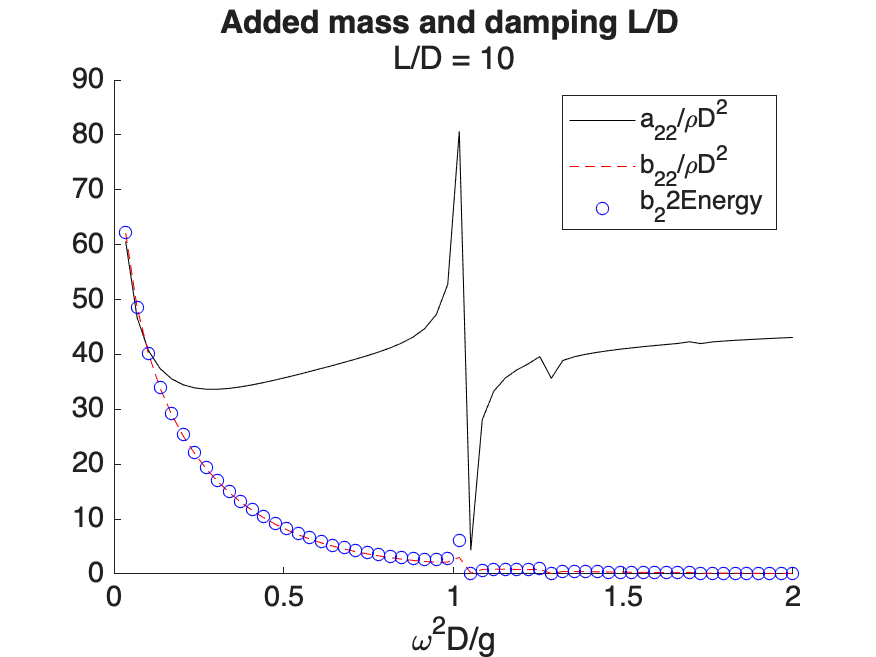
\includegraphics[width=\linewidth]{/Users/ole/Tex/MEK4420/oblig2images/plot_a22b22_1.png}
    \captionof{figure}{L/D = 10}\label{fig:a22_1}
\end{minipage}
\hspace{0.05\linewidth}
\begin{minipage}[t]{0.45\linewidth}
    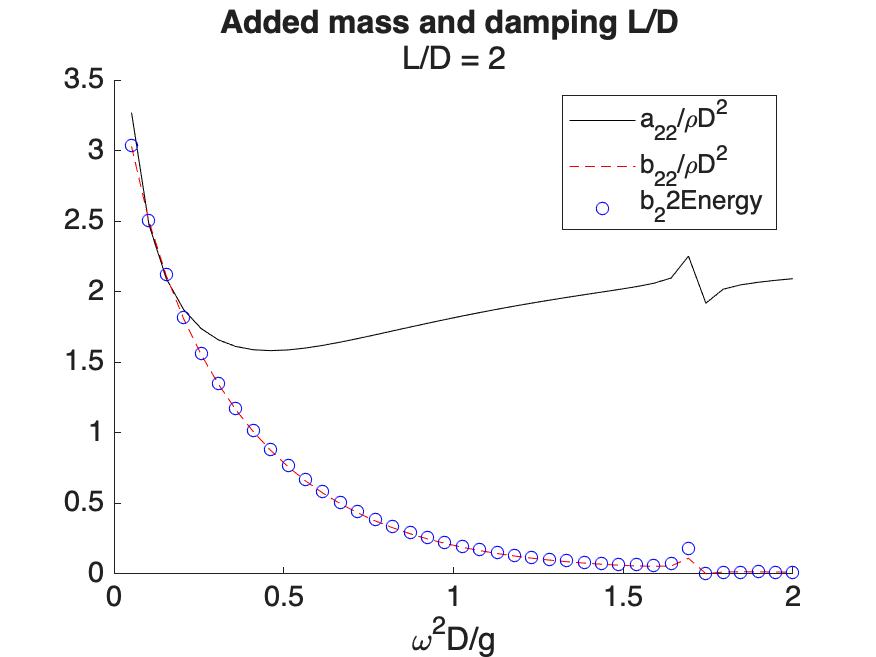
\includegraphics[width=\linewidth]{/Users/ole/Tex/MEK4420/oblig2images/plot_a22b22_2.png}
    \captionof{figure}{L/D = 2}\label{fig:a22_2}
\end{minipage}
\begin{minipage}[t]{0.45\linewidth}
    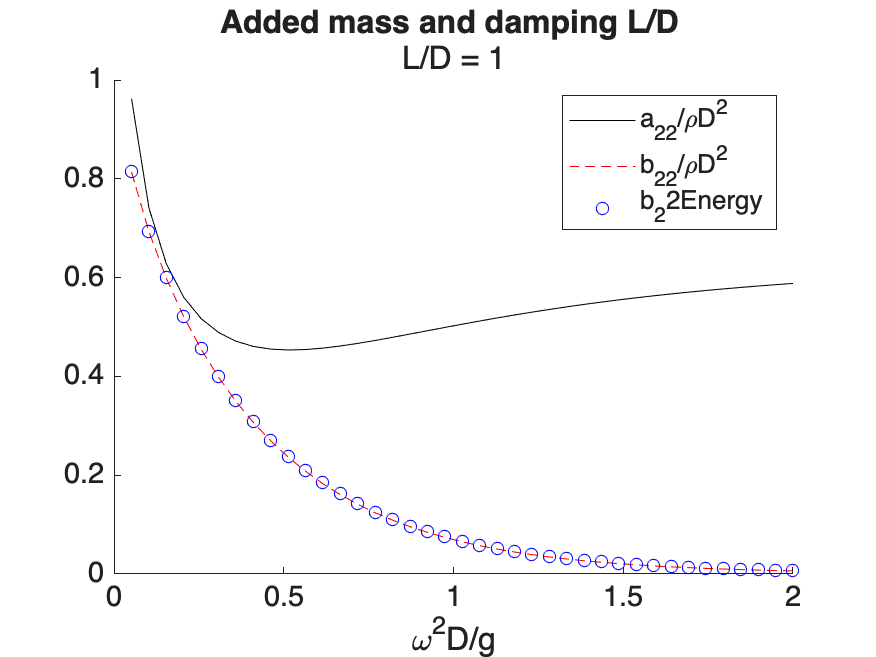
\includegraphics[width=\linewidth]{/Users/ole/Tex/MEK4420/oblig2images/plot_a22b22_3.png}
    \captionof{figure}{L/D = 1}\label{fig:a22_3}
\end{minipage}
\hspace{0.05\linewidth}
\begin{minipage}[t]{0.45\linewidth}
    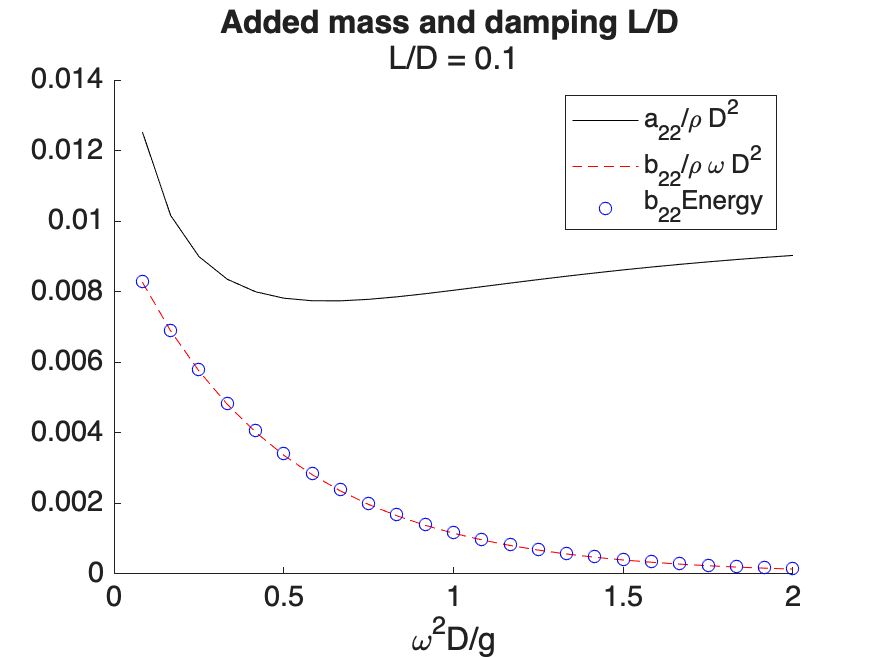
\includegraphics[width=\linewidth]{/Users/ole/Tex/MEK4420/oblig2images/plot_a22b22_4.png}
    \captionof{figure}{L/D = 0.1}\label{fig:a22_4}
\end{minipage} 
\end{frame}

% 7.9 Tilnermet løsning 
\begin{frame}
Vi starter med utgangspunkt i følgende fra Froude-Krylov approksimasjon for å estimere eksitasjonskraften %FK sin approx?
\begin{equation}
	X_2^{FK} = - \mathrm{i} \omega \rho \int_{S_B} \phi_0 n_2 dS =\rho g \int_{-L/2}^{L/2} e^{-KD- \mathrm{i}Kx} dx = \rho g L e^{-KD} \frac{\sin(KL/2)}{KL/2} 
\end{equation}
der $D$ er dypgang og $L$ er lengden. 
%%%%%%med understrek streket ut phi7
%\begin{equation} X_2^{FK} = - \mathrm{i} \omega \rho \int_{S_B} \underbrace{(\phi_0 + \xcancel{\phi_7})}_{FK \text{ ignorerer }\phi_7} n_2 dS = \rho g \int_{-L/2}^{L/2} e^{-KD- \mathrm{i}Kx} dx = \rho g L e^{-KD} \frac{\sin(KL/2)}{KL/2} \end{equation}
Som gir oss
\begin{equation} X_2^{FK} 
 = \rho g L e^{-KD} , \quad \text{ fordi } \frac{\sin(KL/2)}{KL/2} \simeq 1,  \frac{KL}{2} \ll 1
\end{equation}
vi har 
$c_{22} = \rho g L$.
Fra Haskindrelasjonene finner vi dempningskoeffisienten $b_{22}$,
\begin{align}
	 \frac{b_{22}}{\rho \omega} &= \frac{|X_2|^2 }{(\rho g)^2}\\
\end{align}

Vi finner så responsen i hiv. 
\begin{align}
	(c_{22} - &\omega^2(m_{22} + a_{22}) + \mathrm{i}\omega b_{22})\xi_2 = AX_2\\
	 \frac{\xi_{2}}{A} &= \frac{ \frac{g}{g} L e^{-KD} }{( \frac{g}{g} L -  \frac{\omega^2}{g}L D + \mathrm{i}\underbrace{(\frac{\omega^2}{g})}_{=k} L^2 e^{-2KD} }\\
	 \frac{\xi_{2}}{A} &= \frac{ e^{-KD}}{ 1 - K  D + \mathrm{i} K {L} e^{-2KD} }
\end{align}
\end{frame}

% 7.10 - Diffraksjonsproblemet
\begin{frame}
I diffraksjonsproblemet holdes geometrien fast. Fluidets bevegelse er gitt ved hastighetspotensialet

\begin{equation}
\Phi_D(x,y,t) = Re\Big(A  \phi_D(x,y) e^{\mathrm{i} \omega t} \Big), 
\end{equation}
der $A$ er amplituden og $\phi_0$ potensialet til innkommende bølger. Potensialet D finner vi fra $\phi_D(x,y) =  \phi_0(x,y) +  \phi_7(x,y)$. 
$\phi_0(x,y) = \frac{\mathrm{i} g}{\omega}e^{Ky -\mathrm{i} K x}$. Og $K = \frac{\omega^2}{g}$. Spredningen $\phi_7$ er ukjent.

Integrallikningen vi bruker for å bestemme summen $\phi_D =  \phi_0 +  \phi_7$ til et punkt $(\bar{x},\bar{y})$ på $S_B$ er
\begin{equation}
    -\pi \phi_D(\bar{x},\bar{y})  + \int_{S_B}   \phi_D  \frac{\partial G }{\partial n}dS = -2\pi \phi_0(\bar{x},\bar{y}) 
\end{equation}
\end{frame}

% 7.10 1og2. Eksitasjonskraft og Haskind.
\begin{frame}
Vi ønsker å finne påvirkningskraften numerisk. 
\begin{equation}
\frac{X_2}{\rho g}  =  -  \frac{\mathrm{i} \omega}{g}\int_{S_B}   \phi_D n_2dS
%HOPPER OVER HASKIND FORELØPIG
\end{equation}
\end{frame}

%SAMMENLIKNE EKSITASJONSKRAFT, HASKIND 1&2 OG FROUDE-KRYLOV
\begin{frame}
haskind, FK, 
\end{frame}

% 7.11 Respons i hiv -likning
\begin{frame}
Likning for bevegelsen, kun i hiv, er gitt ved
\begin{equation}
( - \omega^2(m+a_{22}) + \mathrm{i}\omega b_{22}+ c_{22})\xi_2 = AX_2, 
\end{equation}
\begin{equation}
\frac{|\xi_2|}{A} = \frac{X_2}{c_{22} - \omega^2(m+a_{22}) + \mathrm{i}\omega b_{22}}, 
\end{equation}
der $c_{22} = \rho g S$. Svømmeflaten $S$ i vårt todimensjonale tilfelle er lengden på geometrien. $m$ er massen til geometrien, som for et fritt flytende legme er lik oppdriftskraften. Den adderte massen blir $a_{22} = \rho \forall = \rho LD$. $b_{22}$ er
\begin{equation}
b_{22} = \frac{K }{4\rho g V_g}|X_2|^2. 
\end{equation}
\end{frame}

% 7.11.1 Respons i hiv  - resonans. 
\begin{frame}
Resonansfrekvensen $\omega_n$ oppstår der de hydrostatiske kreftene balanserer treghetskreftene, $c_{22}-\omega^2(m+a_{22}) = 0$. Resonansfrekvensen for en fritt flytende todimensjonal rektangulær seksjon med bredde L og dypgang D=1 blir, 

\begin{equation}
\omega^2_n = \frac{g}{D}  \frac{1}{1 + \frac{a_{22}}{\rho DL}}, 
\end{equation}
%For våre 4 geometrier finner vi addert masse fra figur \ref{fig:a22_1}, \ref{fig:a22_2}, \ref{fig:a22_3} og \ref{fig:a22_4}. 

\begin{table}[htp]
\centering
\renewcommand{\arraystretch}{1.3} % Slightly increases row height
\caption{Resonansfrekvens}
\label{default}
\begin{tabular}{|p{1cm}|p{1cm}|p{1cm}|p{1cm}|p{1cm}|}
\hline
L/D & 10 & 2 & 1 & 0.1 \\ \hline
$a_{22}$ & 40 & 1.8 & 0.5 & 0.009 \\ \hline
$\frac{w_n^2}{g}$ & 0.2 & 0.53 & 0.67 & 0.92 \\ \hline
\end{tabular}
\end{table}
\end{frame}

% 7.11.2-3-4 Response as a function of frequency
\begin{frame}
%section{7.11.3}%section{7.11.4}%7.11.2-3-4 gir ett plott.
%Vi plotter responsen $\frac{|\xi|}{A}$ på tre måter. Først som en funksjon av frekvensen. Så, funnet ved Froude-Krylov-approksimasjonen $X_2^{FK}$, der $b_{22}$ finnes ved Haskind-relasjonene, og der effekten av addert masse $a_{22}$ er ignorert. Og til slutt, approksimasjonen, men justert for addert masse. Vi ser at verdiene for resonansfrekvensen tilsvarer toppene på kurvene våre.

\noindent
\begin{minipage}[t]{0.45\linewidth}
    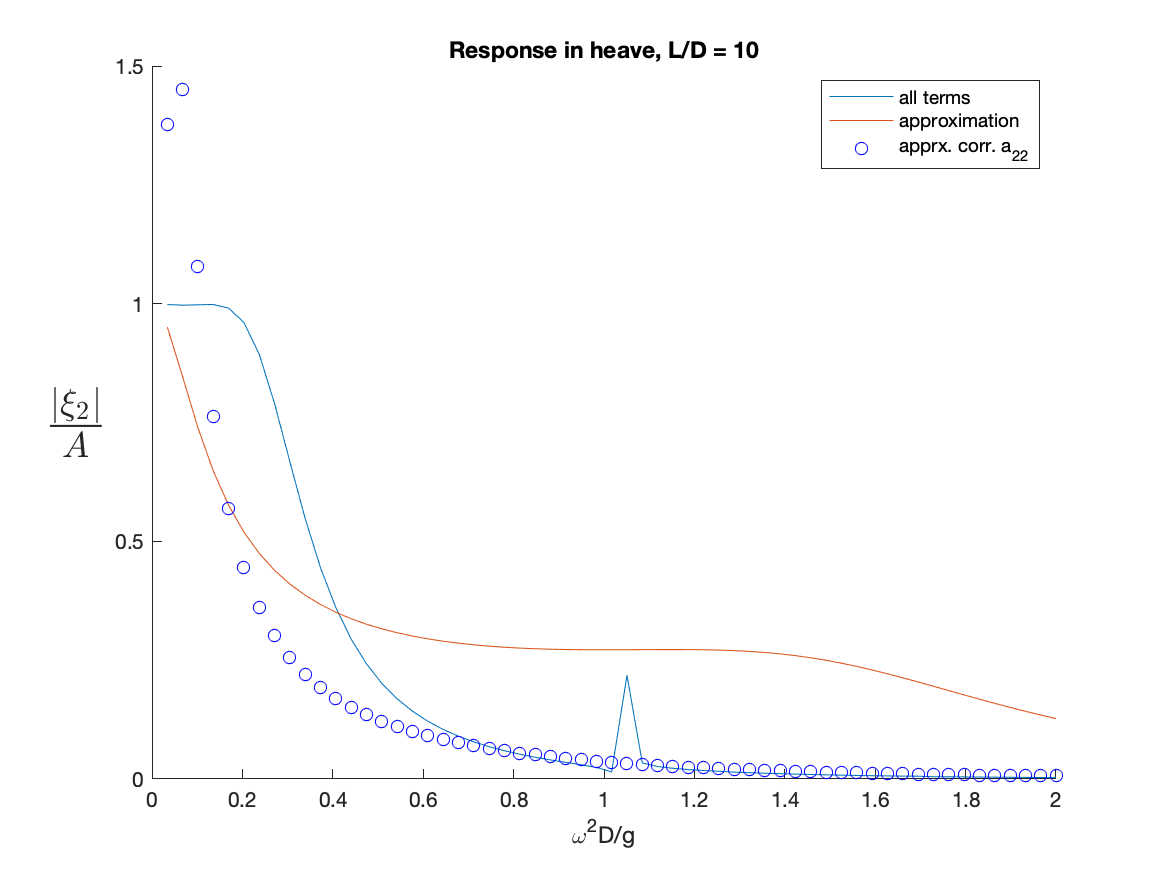
\includegraphics[width=\linewidth]{/Users/ole/Tex/MEK4420/oblig2images/rao_plot1_LD_1.png}
    \captionof{figure}{L/D = 10}
\end{minipage}
\hspace{0.05\linewidth}
\begin{minipage}[t]{0.45\linewidth}
    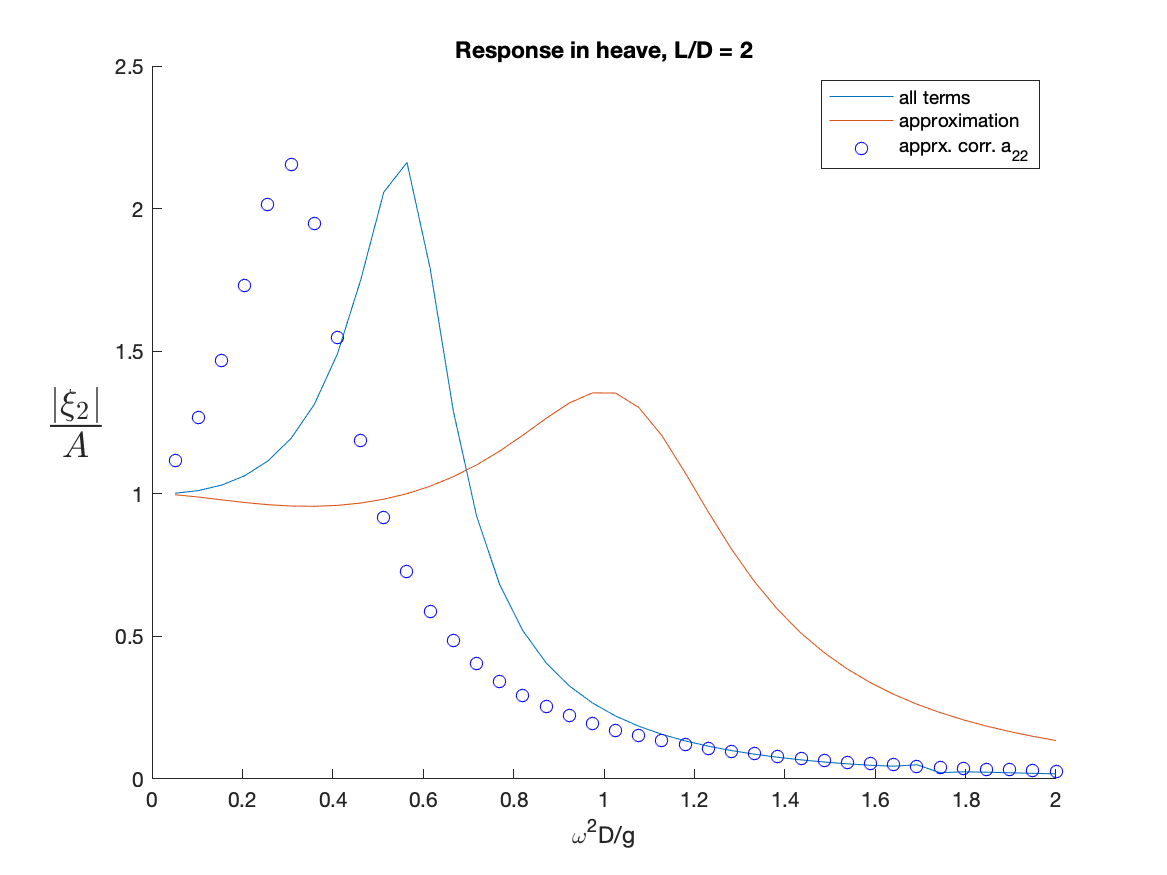
\includegraphics[width=\linewidth]{/Users/ole/Tex/MEK4420/oblig2images/rao_plot2_LD_2.png}
    \captionof{figure}{L/D = 2}
\end{minipage}
\noindent
\begin{minipage}[t]{0.45\linewidth}
    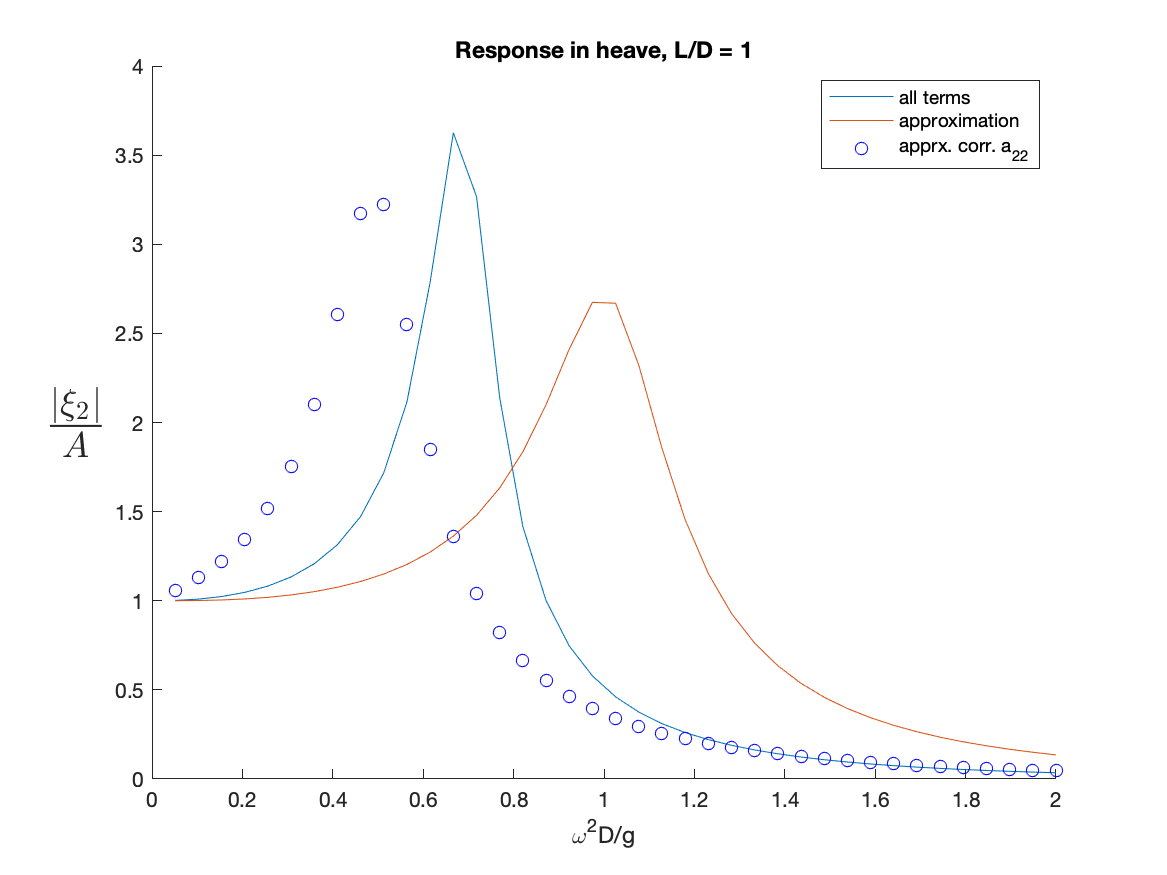
\includegraphics[width=\linewidth]{/Users/ole/Tex/MEK4420/oblig2images/rao_plot3_LD_3.png}
    \captionof{figure}{L/D = 1}
\end{minipage}
\hspace{0.05\linewidth}
\begin{minipage}[t]{0.45\linewidth}
    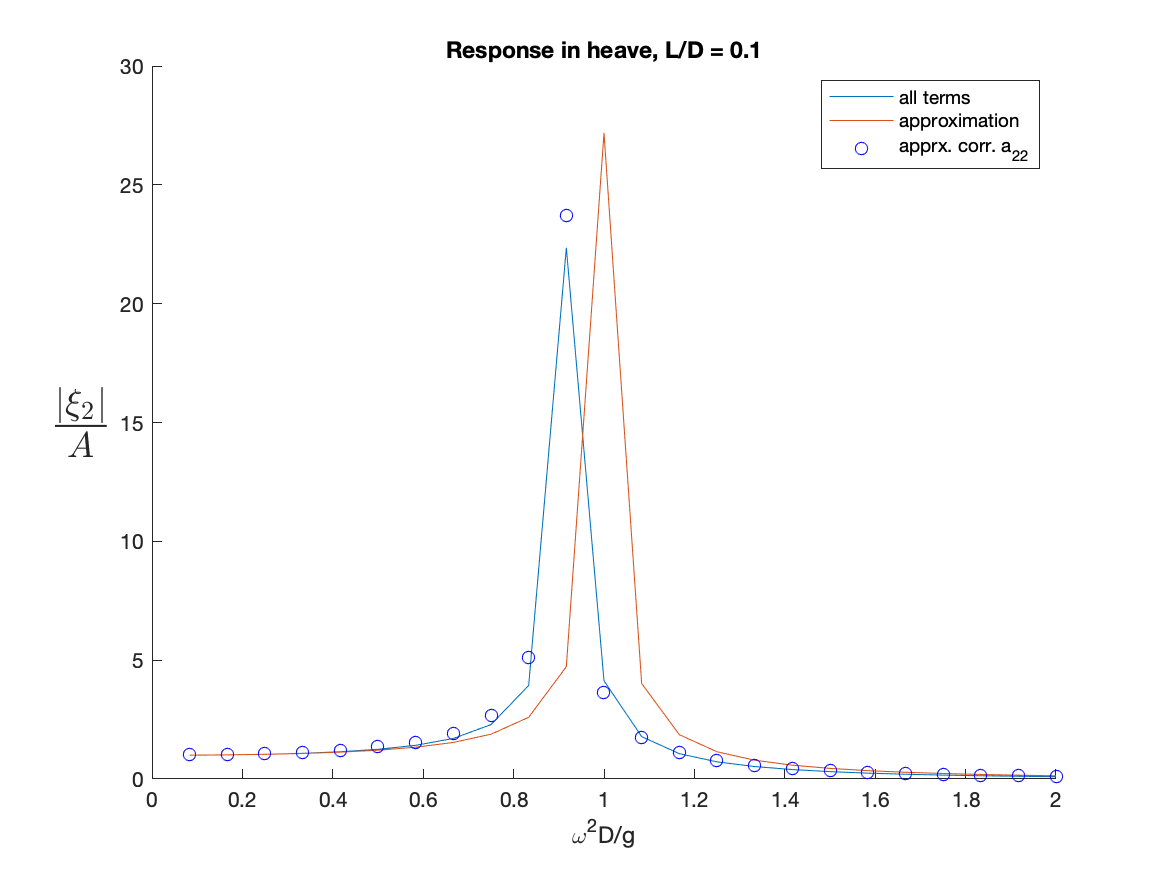
\includegraphics[width=\linewidth]{/Users/ole/Tex/MEK4420/oblig2images/rao_plot4_LD_4.png}
    \captionof{figure}{L/D = 0.1}
\end{minipage}
\end{frame}

% 
\begin{frame}
slutt
\end{frame}

\end{document}
